\documentclass[twoside]{book}

% Packages required by doxygen
\usepackage{fixltx2e}
\usepackage{calc}
\usepackage{doxygen}
\usepackage[export]{adjustbox} % also loads graphicx
\usepackage{graphicx}
\usepackage[utf8]{inputenc}
\usepackage{makeidx}
\usepackage{multicol}
\usepackage{multirow}
\PassOptionsToPackage{warn}{textcomp}
\usepackage{textcomp}
\usepackage[nointegrals]{wasysym}
\usepackage[table]{xcolor}

% Font selection
\usepackage[T1]{fontenc}
\usepackage[scaled=.90]{helvet}
\usepackage{courier}
\usepackage{amssymb}
\usepackage{sectsty}
\renewcommand{\familydefault}{\sfdefault}
\allsectionsfont{%
  \fontseries{bc}\selectfont%
  \color{darkgray}%
}
\renewcommand{\DoxyLabelFont}{%
  \fontseries{bc}\selectfont%
  \color{darkgray}%
}
\newcommand{\+}{\discretionary{\mbox{\scriptsize$\hookleftarrow$}}{}{}}

% Page & text layout
\usepackage{geometry}
\geometry{%
  a4paper,%
  top=2.5cm,%
  bottom=2.5cm,%
  left=2.5cm,%
  right=2.5cm%
}
\tolerance=750
\hfuzz=15pt
\hbadness=750
\setlength{\emergencystretch}{15pt}
\setlength{\parindent}{0cm}
\setlength{\parskip}{3ex plus 2ex minus 2ex}
\makeatletter
\renewcommand{\paragraph}{%
  \@startsection{paragraph}{4}{0ex}{-1.0ex}{1.0ex}{%
    \normalfont\normalsize\bfseries\SS@parafont%
  }%
}
\renewcommand{\subparagraph}{%
  \@startsection{subparagraph}{5}{0ex}{-1.0ex}{1.0ex}{%
    \normalfont\normalsize\bfseries\SS@subparafont%
  }%
}
\makeatother

% Headers & footers
\usepackage{fancyhdr}
\pagestyle{fancyplain}
\fancyhead[LE]{\fancyplain{}{\bfseries\thepage}}
\fancyhead[CE]{\fancyplain{}{}}
\fancyhead[RE]{\fancyplain{}{\bfseries\leftmark}}
\fancyhead[LO]{\fancyplain{}{\bfseries\rightmark}}
\fancyhead[CO]{\fancyplain{}{}}
\fancyhead[RO]{\fancyplain{}{\bfseries\thepage}}
\fancyfoot[LE]{\fancyplain{}{}}
\fancyfoot[CE]{\fancyplain{}{}}
\fancyfoot[RE]{\fancyplain{}{\bfseries\scriptsize Generated by Doxygen }}
\fancyfoot[LO]{\fancyplain{}{\bfseries\scriptsize Generated by Doxygen }}
\fancyfoot[CO]{\fancyplain{}{}}
\fancyfoot[RO]{\fancyplain{}{}}
\renewcommand{\footrulewidth}{0.4pt}
\renewcommand{\chaptermark}[1]{%
  \markboth{#1}{}%
}
\renewcommand{\sectionmark}[1]{%
  \markright{\thesection\ #1}%
}

% Indices & bibliography
\usepackage{natbib}
\usepackage[titles]{tocloft}
\setcounter{tocdepth}{3}
\setcounter{secnumdepth}{5}
\makeindex

% Hyperlinks (required, but should be loaded last)
\usepackage{ifpdf}
\ifpdf
  \usepackage[pdftex,pagebackref=true]{hyperref}
\else
  \usepackage[ps2pdf,pagebackref=true]{hyperref}
\fi
\hypersetup{%
  colorlinks=true,%
  linkcolor=blue,%
  citecolor=blue,%
  unicode%
}

% Custom commands
\newcommand{\clearemptydoublepage}{%
  \newpage{\pagestyle{empty}\cleardoublepage}%
}

\usepackage{caption}
\captionsetup{labelsep=space,justification=centering,font={bf},singlelinecheck=off,skip=4pt,position=top}

%===== C O N T E N T S =====

\begin{document}

% Titlepage & ToC
\hypersetup{pageanchor=false,
             bookmarksnumbered=true,
             pdfencoding=unicode
            }
\pagenumbering{alph}
\begin{titlepage}
\vspace*{7cm}
\begin{center}%
{\Large My Project }\\
\vspace*{1cm}
{\large Generated by Doxygen 1.8.14}\\
\end{center}
\end{titlepage}
\clearemptydoublepage
\pagenumbering{roman}
\tableofcontents
\clearemptydoublepage
\pagenumbering{arabic}
\hypersetup{pageanchor=true}

%--- Begin generated contents ---
\chapter{Closet\+Plus\+Plus}
\label{md_README}
\Hypertarget{md_README}
\input{md_README}
\chapter{Hierarchical Index}
\section{Class Hierarchy}
This inheritance list is sorted roughly, but not completely, alphabetically\+:\begin{DoxyCompactList}
\item \contentsline{section}{Closet}{\pageref{classCloset}}{}
\item \contentsline{section}{Clothes}{\pageref{classClothes}}{}
\begin{DoxyCompactList}
\item \contentsline{section}{Belt}{\pageref{classBelt}}{}
\item \contentsline{section}{Pants}{\pageref{classPants}}{}
\item \contentsline{section}{Shirt}{\pageref{classShirt}}{}
\item \contentsline{section}{Shoes}{\pageref{classShoes}}{}
\item \contentsline{section}{Socks}{\pageref{classSocks}}{}
\end{DoxyCompactList}
\item \contentsline{section}{Ncurses}{\pageref{classNcurses}}{}
\item \contentsline{section}{Window}{\pageref{classWindow}}{}
\begin{DoxyCompactList}
\item \contentsline{section}{Vulkan}{\pageref{classVulkan}}{}
\end{DoxyCompactList}
\end{DoxyCompactList}

\chapter{Class Index}
\section{Class List}
Here are the classes, structs, unions and interfaces with brief descriptions\+:\begin{DoxyCompactList}
\item\contentsline{section}{\mbox{\hyperlink{classBelt}{Belt}} }{\pageref{classBelt}}{}
\item\contentsline{section}{\mbox{\hyperlink{classCloset}{Closet}} }{\pageref{classCloset}}{}
\item\contentsline{section}{\mbox{\hyperlink{classClothes}{Clothes}} }{\pageref{classClothes}}{}
\item\contentsline{section}{\mbox{\hyperlink{classNcurses}{Ncurses}} }{\pageref{classNcurses}}{}
\item\contentsline{section}{\mbox{\hyperlink{classPants}{Pants}} }{\pageref{classPants}}{}
\item\contentsline{section}{\mbox{\hyperlink{classShirt}{Shirt}} }{\pageref{classShirt}}{}
\item\contentsline{section}{\mbox{\hyperlink{classShoes}{Shoes}} }{\pageref{classShoes}}{}
\item\contentsline{section}{\mbox{\hyperlink{classSocks}{Socks}} }{\pageref{classSocks}}{}
\item\contentsline{section}{\mbox{\hyperlink{classVulkan}{Vulkan}} }{\pageref{classVulkan}}{}
\item\contentsline{section}{\mbox{\hyperlink{classWindow}{Window}} }{\pageref{classWindow}}{}
\end{DoxyCompactList}

\chapter{Class Documentation}
\hypertarget{classBelt}{}\section{Belt Class Reference}
\label{classBelt}\index{Belt@{Belt}}


{\ttfamily \#include \char`\"{}belt.\+h\char`\"{}}



Inheritance diagram for Belt\+:\nopagebreak
\begin{figure}[H]
\begin{center}
\leavevmode
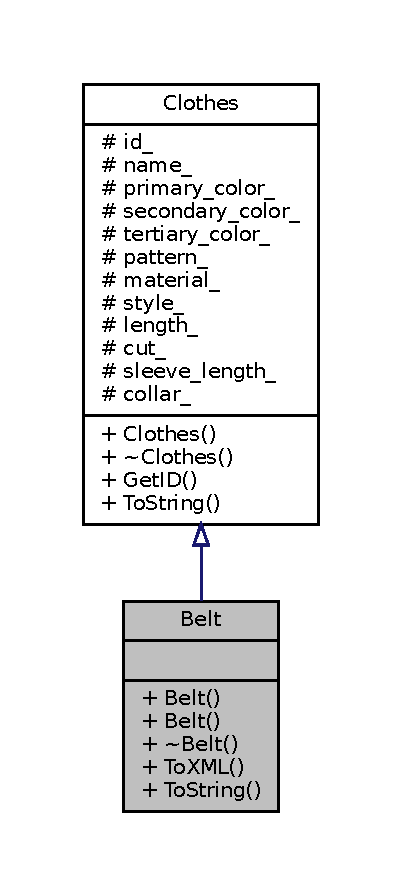
\includegraphics[width=193pt]{classBelt__inherit__graph}
\end{center}
\end{figure}


Collaboration diagram for Belt\+:\nopagebreak
\begin{figure}[H]
\begin{center}
\leavevmode
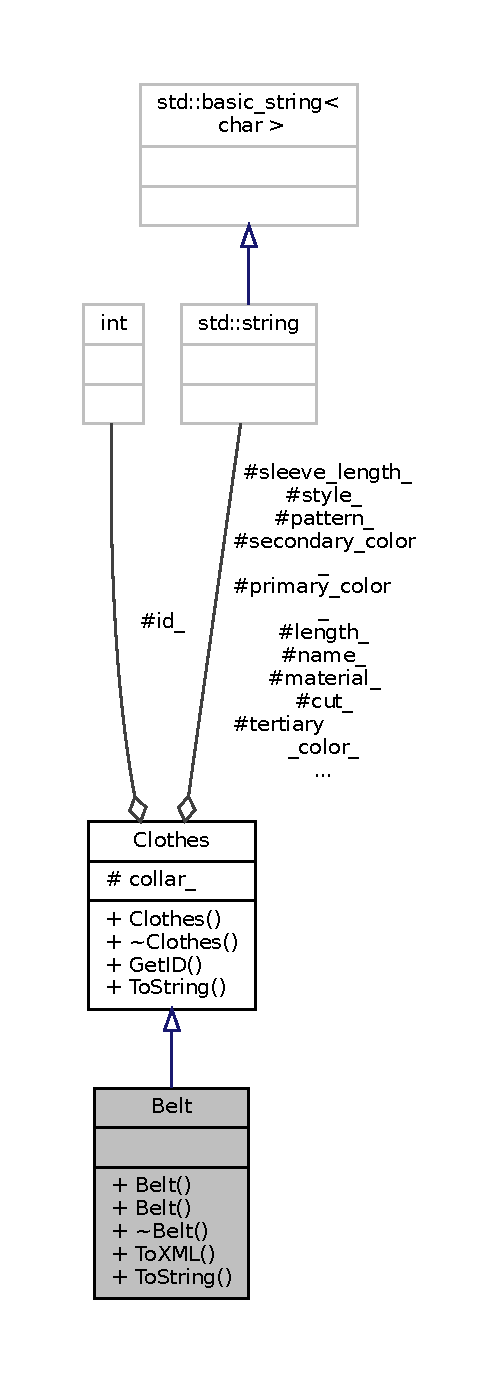
\includegraphics[height=550pt]{classBelt__coll__graph}
\end{center}
\end{figure}
\subsection*{Public Member Functions}
\begin{DoxyCompactItemize}
\item 
\mbox{\hyperlink{classBelt_a6dc40c21b5a62c71925df189511d7551}{Belt}} ()
\item 
\mbox{\hyperlink{classBelt_a2a8b481a0fe80916513dbd5cf1f03127}{Belt}} (int id, string name, string prim\+\_\+color, string sec\+\_\+color, string tert\+\_\+color, string material, string pattern)
\item 
virtual \mbox{\hyperlink{classBelt_a671f01a32839b9391d75ae3bb0b7f8cc}{$\sim$\+Belt}} ()
\item 
string \mbox{\hyperlink{classBelt_a69b84739e63f35afa5dacf6f3ce0d731}{To\+X\+ML}} () const
\item 
string \mbox{\hyperlink{classBelt_af09e2b5e51b7603ec5dede2e6b0a753f}{To\+String}} () const
\item 
int \mbox{\hyperlink{classClothes_a3f6dac172f333126d19010f85ec44e4c}{Get\+ID}} ()
\end{DoxyCompactItemize}
\subsection*{Protected Attributes}
\begin{DoxyCompactItemize}
\item 
int \mbox{\hyperlink{classClothes_a8978d931db5ca47c3ccea30def4ae83e}{id\+\_\+}} = \mbox{\hyperlink{clothes_8h_a77186917343a417a2369cdff0bc86d31}{k\+Dummy\+ID}}
\begin{DoxyCompactList}\small\item\em Global unique identifier. \end{DoxyCompactList}\item 
string \mbox{\hyperlink{classClothes_a7f2275aaae24224d60c48af922c31b65}{name\+\_\+}} = \mbox{\hyperlink{clothes_8h_adba739b5125fd5a4066ec0ef063c0657}{k\+Dummy\+Name}}
\begin{DoxyCompactList}\small\item\em User readable name. \end{DoxyCompactList}\item 
string \mbox{\hyperlink{classClothes_a7cb005bf6cbb7f4eaa40f1b31817559c}{primary\+\_\+color\+\_\+}} = \mbox{\hyperlink{clothes_8h_a1b9c685d3bf2811d95b65e0d396c1344}{k\+Dummy\+Prim\+Color}}
\begin{DoxyCompactList}\small\item\em Primary color. \end{DoxyCompactList}\item 
string \mbox{\hyperlink{classClothes_ab8f55f67b956b25d71260cffcf273673}{secondary\+\_\+color\+\_\+}} = \mbox{\hyperlink{clothes_8h_a71c39811135425d881af7760da63a73a}{k\+Dummy\+Sec\+Color}}
\begin{DoxyCompactList}\small\item\em Secondary color. \end{DoxyCompactList}\item 
string \mbox{\hyperlink{classClothes_a3c5f1e7ab531e3ba7a38b930da8078a0}{tertiary\+\_\+color\+\_\+}} = \mbox{\hyperlink{clothes_8h_a094dde85547895fd70dafb3ab10c6783}{k\+Dummy\+Tert\+Color}}
\begin{DoxyCompactList}\small\item\em Tertiary color. \end{DoxyCompactList}\item 
string \mbox{\hyperlink{classClothes_a1d40145a4eb6d28441f112f030ab5d35}{pattern\+\_\+}} = \mbox{\hyperlink{clothes_8h_a2e72ae4d77adb7bc9cbecf4dea1e9e22}{k\+Dummy\+Pattern}}
\begin{DoxyCompactList}\small\item\em Design pattern. \end{DoxyCompactList}\item 
string \mbox{\hyperlink{classClothes_adbb9ed311f14ccbb1e4fe0e8378a95d4}{material\+\_\+}} = \mbox{\hyperlink{clothes_8h_a9df1268c6668ae4e2a728ccf032cc33d}{k\+Dummy\+Material}}
\begin{DoxyCompactList}\small\item\em Material. \end{DoxyCompactList}\item 
string \mbox{\hyperlink{classClothes_aa85ed2b95110d8c477a1aca9cb403f98}{style\+\_\+}} = \mbox{\hyperlink{clothes_8h_a9deec6ed1f40928bfa0040eeab95ed6b}{k\+Dummy\+Style}}
\begin{DoxyCompactList}\small\item\em Design style. \end{DoxyCompactList}\item 
string \mbox{\hyperlink{classClothes_ae02603eda727e33caf46ec30e761e3c3}{length\+\_\+}} = \mbox{\hyperlink{clothes_8h_a1624256dcecfb0995a74c36142593770}{k\+Dummy\+Length}}
\begin{DoxyCompactList}\small\item\em Length of the clothing. \end{DoxyCompactList}\item 
string \mbox{\hyperlink{classClothes_ac1c2286c8928a5eee91d818a098a44ac}{cut\+\_\+}} = \mbox{\hyperlink{clothes_8h_a8a6eb066049b009439505355aeaae375}{k\+Dummy\+Cut}}
\begin{DoxyCompactList}\small\item\em Cut of the clothing. \end{DoxyCompactList}\item 
string \mbox{\hyperlink{classClothes_a012aeb71e62ebaf9b5b5dd700cc8d5db}{sleeve\+\_\+length\+\_\+}} = \mbox{\hyperlink{clothes_8h_a0f53dde6a2c4c344bb7da50655497350}{k\+Dummy\+Sleeve\+Length}}
\begin{DoxyCompactList}\small\item\em Length of the sleeve. \end{DoxyCompactList}\item 
string \mbox{\hyperlink{classClothes_ae2e5026257b3a2f2ddbf61757fd3b57b}{collar\+\_\+}} = \mbox{\hyperlink{clothes_8h_ac06c9f556f68bcd2829e36c55b70a86e}{k\+Dummy\+Collar}}
\begin{DoxyCompactList}\small\item\em Type of collar. \end{DoxyCompactList}\end{DoxyCompactItemize}


\subsection{Detailed Description}
\begin{DoxyAuthor}{Author}
Stephen M. Reaves 
\end{DoxyAuthor}
\begin{DoxyDate}{Date}
July 14th, 2018 
\end{DoxyDate}


\subsection{Constructor \& Destructor Documentation}
\mbox{\Hypertarget{classBelt_a6dc40c21b5a62c71925df189511d7551}\label{classBelt_a6dc40c21b5a62c71925df189511d7551}} 
\index{Belt@{Belt}!Belt@{Belt}}
\index{Belt@{Belt}!Belt@{Belt}}
\subsubsection{\texorpdfstring{Belt()}{Belt()}\hspace{0.1cm}{\footnotesize\ttfamily [1/2]}}
{\footnotesize\ttfamily Belt\+::\+Belt (\begin{DoxyParamCaption}{ }\end{DoxyParamCaption})}

Default Constructor

\begin{DoxyReturn}{Returns}
\mbox{\hyperlink{classBelt}{Belt}} Object 
\end{DoxyReturn}
\mbox{\Hypertarget{classBelt_a2a8b481a0fe80916513dbd5cf1f03127}\label{classBelt_a2a8b481a0fe80916513dbd5cf1f03127}} 
\index{Belt@{Belt}!Belt@{Belt}}
\index{Belt@{Belt}!Belt@{Belt}}
\subsubsection{\texorpdfstring{Belt()}{Belt()}\hspace{0.1cm}{\footnotesize\ttfamily [2/2]}}
{\footnotesize\ttfamily Belt\+::\+Belt (\begin{DoxyParamCaption}\item[{int}]{id,  }\item[{string}]{name,  }\item[{string}]{prim\+\_\+color,  }\item[{string}]{sec\+\_\+color,  }\item[{string}]{tert\+\_\+color,  }\item[{string}]{material,  }\item[{string}]{pattern }\end{DoxyParamCaption})}

Parameterized Constructor


\begin{DoxyParams}{Parameters}
{\em id} & Integer uniquely identifying this object across the whole closet \\
\hline
{\em name} & String used to inentify this object to the user \\
\hline
{\em prim\+\_\+color} & Primary color of this belt \\
\hline
{\em sec\+\_\+color} & Secondary color of this belt \\
\hline
{\em tert\+\_\+color} & Tertiary color of this belt \\
\hline
{\em material} & Material this belt is made of \\
\hline
{\em pattern} & Design pattern of this belt\\
\hline
\end{DoxyParams}
\begin{DoxyReturn}{Returns}
\mbox{\hyperlink{classBelt}{Belt}} Object 
\end{DoxyReturn}


References \mbox{\hyperlink{classClothes_a8978d931db5ca47c3ccea30def4ae83e}{Clothes\+::id\+\_\+}}, \mbox{\hyperlink{classClothes_adbb9ed311f14ccbb1e4fe0e8378a95d4}{Clothes\+::material\+\_\+}}, \mbox{\hyperlink{classClothes_a7f2275aaae24224d60c48af922c31b65}{Clothes\+::name\+\_\+}}, \mbox{\hyperlink{classClothes_a1d40145a4eb6d28441f112f030ab5d35}{Clothes\+::pattern\+\_\+}}, \mbox{\hyperlink{classClothes_a7cb005bf6cbb7f4eaa40f1b31817559c}{Clothes\+::primary\+\_\+color\+\_\+}}, \mbox{\hyperlink{classClothes_ab8f55f67b956b25d71260cffcf273673}{Clothes\+::secondary\+\_\+color\+\_\+}}, and \mbox{\hyperlink{classClothes_a3c5f1e7ab531e3ba7a38b930da8078a0}{Clothes\+::tertiary\+\_\+color\+\_\+}}.

\mbox{\Hypertarget{classBelt_a671f01a32839b9391d75ae3bb0b7f8cc}\label{classBelt_a671f01a32839b9391d75ae3bb0b7f8cc}} 
\index{Belt@{Belt}!````~Belt@{$\sim$\+Belt}}
\index{````~Belt@{$\sim$\+Belt}!Belt@{Belt}}
\subsubsection{\texorpdfstring{$\sim$\+Belt()}{~Belt()}}
{\footnotesize\ttfamily Belt\+::$\sim$\+Belt (\begin{DoxyParamCaption}{ }\end{DoxyParamCaption})\hspace{0.3cm}{\ttfamily [virtual]}}

Deconstructor 

\subsection{Member Function Documentation}
\mbox{\Hypertarget{classClothes_a3f6dac172f333126d19010f85ec44e4c}\label{classClothes_a3f6dac172f333126d19010f85ec44e4c}} 
\index{Belt@{Belt}!Get\+ID@{Get\+ID}}
\index{Get\+ID@{Get\+ID}!Belt@{Belt}}
\subsubsection{\texorpdfstring{Get\+I\+D()}{GetID()}}
{\footnotesize\ttfamily int Clothes\+::\+Get\+ID (\begin{DoxyParamCaption}{ }\end{DoxyParamCaption})\hspace{0.3cm}{\ttfamily [inline]}, {\ttfamily [inherited]}}

Here is the caller graph for this function\+:\nopagebreak
\begin{figure}[H]
\begin{center}
\leavevmode
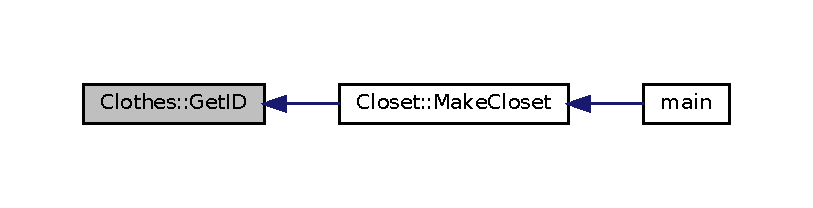
\includegraphics[width=350pt]{classClothes_a3f6dac172f333126d19010f85ec44e4c_icgraph}
\end{center}
\end{figure}
\mbox{\Hypertarget{classBelt_af09e2b5e51b7603ec5dede2e6b0a753f}\label{classBelt_af09e2b5e51b7603ec5dede2e6b0a753f}} 
\index{Belt@{Belt}!To\+String@{To\+String}}
\index{To\+String@{To\+String}!Belt@{Belt}}
\subsubsection{\texorpdfstring{To\+String()}{ToString()}}
{\footnotesize\ttfamily string Belt\+::\+To\+String (\begin{DoxyParamCaption}{ }\end{DoxyParamCaption}) const\hspace{0.3cm}{\ttfamily [virtual]}}

To\+String \begin{DoxyReturn}{Returns}
\textquotesingle{}string\textquotesingle{} representing the belt. 
\end{DoxyReturn}


Implements \mbox{\hyperlink{classClothes_a953d143394e9a2c007ab0c3a638973cf}{Clothes}}.



References \mbox{\hyperlink{classClothes_a8978d931db5ca47c3ccea30def4ae83e}{Clothes\+::id\+\_\+}}, \mbox{\hyperlink{classClothes_adbb9ed311f14ccbb1e4fe0e8378a95d4}{Clothes\+::material\+\_\+}}, \mbox{\hyperlink{classClothes_a7f2275aaae24224d60c48af922c31b65}{Clothes\+::name\+\_\+}}, \mbox{\hyperlink{classClothes_a1d40145a4eb6d28441f112f030ab5d35}{Clothes\+::pattern\+\_\+}}, \mbox{\hyperlink{classClothes_a7cb005bf6cbb7f4eaa40f1b31817559c}{Clothes\+::primary\+\_\+color\+\_\+}}, \mbox{\hyperlink{classClothes_ab8f55f67b956b25d71260cffcf273673}{Clothes\+::secondary\+\_\+color\+\_\+}}, and \mbox{\hyperlink{classClothes_a3c5f1e7ab531e3ba7a38b930da8078a0}{Clothes\+::tertiary\+\_\+color\+\_\+}}.

\mbox{\Hypertarget{classBelt_a69b84739e63f35afa5dacf6f3ce0d731}\label{classBelt_a69b84739e63f35afa5dacf6f3ce0d731}} 
\index{Belt@{Belt}!To\+X\+ML@{To\+X\+ML}}
\index{To\+X\+ML@{To\+X\+ML}!Belt@{Belt}}
\subsubsection{\texorpdfstring{To\+X\+M\+L()}{ToXML()}}
{\footnotesize\ttfamily string Belt\+::\+To\+X\+ML (\begin{DoxyParamCaption}{ }\end{DoxyParamCaption}) const}

To\+X\+ML \begin{DoxyRefDesc}{Deprecated}
\item[\mbox{\hyperlink{deprecated__deprecated000001}{Deprecated}}]\end{DoxyRefDesc}
\begin{DoxyReturn}{Returns}
X\+ML representing the belt. 
\end{DoxyReturn}


References \mbox{\hyperlink{classClothes_a8978d931db5ca47c3ccea30def4ae83e}{Clothes\+::id\+\_\+}}, \mbox{\hyperlink{classClothes_adbb9ed311f14ccbb1e4fe0e8378a95d4}{Clothes\+::material\+\_\+}}, \mbox{\hyperlink{classClothes_a7f2275aaae24224d60c48af922c31b65}{Clothes\+::name\+\_\+}}, \mbox{\hyperlink{classClothes_a7cb005bf6cbb7f4eaa40f1b31817559c}{Clothes\+::primary\+\_\+color\+\_\+}}, \mbox{\hyperlink{classClothes_ab8f55f67b956b25d71260cffcf273673}{Clothes\+::secondary\+\_\+color\+\_\+}}, and \mbox{\hyperlink{classClothes_a3c5f1e7ab531e3ba7a38b930da8078a0}{Clothes\+::tertiary\+\_\+color\+\_\+}}.



\subsection{Member Data Documentation}
\mbox{\Hypertarget{classClothes_ae2e5026257b3a2f2ddbf61757fd3b57b}\label{classClothes_ae2e5026257b3a2f2ddbf61757fd3b57b}} 
\index{Belt@{Belt}!collar\+\_\+@{collar\+\_\+}}
\index{collar\+\_\+@{collar\+\_\+}!Belt@{Belt}}
\subsubsection{\texorpdfstring{collar\+\_\+}{collar\_}}
{\footnotesize\ttfamily string Clothes\+::collar\+\_\+ = \mbox{\hyperlink{clothes_8h_ac06c9f556f68bcd2829e36c55b70a86e}{k\+Dummy\+Collar}}\hspace{0.3cm}{\ttfamily [protected]}, {\ttfamily [inherited]}}



Type of collar. 

\mbox{\Hypertarget{classClothes_ac1c2286c8928a5eee91d818a098a44ac}\label{classClothes_ac1c2286c8928a5eee91d818a098a44ac}} 
\index{Belt@{Belt}!cut\+\_\+@{cut\+\_\+}}
\index{cut\+\_\+@{cut\+\_\+}!Belt@{Belt}}
\subsubsection{\texorpdfstring{cut\+\_\+}{cut\_}}
{\footnotesize\ttfamily string Clothes\+::cut\+\_\+ = \mbox{\hyperlink{clothes_8h_a8a6eb066049b009439505355aeaae375}{k\+Dummy\+Cut}}\hspace{0.3cm}{\ttfamily [protected]}, {\ttfamily [inherited]}}



Cut of the clothing. 

\mbox{\Hypertarget{classClothes_a8978d931db5ca47c3ccea30def4ae83e}\label{classClothes_a8978d931db5ca47c3ccea30def4ae83e}} 
\index{Belt@{Belt}!id\+\_\+@{id\+\_\+}}
\index{id\+\_\+@{id\+\_\+}!Belt@{Belt}}
\subsubsection{\texorpdfstring{id\+\_\+}{id\_}}
{\footnotesize\ttfamily int Clothes\+::id\+\_\+ = \mbox{\hyperlink{clothes_8h_a77186917343a417a2369cdff0bc86d31}{k\+Dummy\+ID}}\hspace{0.3cm}{\ttfamily [protected]}, {\ttfamily [inherited]}}



Global unique identifier. 

\mbox{\Hypertarget{classClothes_ae02603eda727e33caf46ec30e761e3c3}\label{classClothes_ae02603eda727e33caf46ec30e761e3c3}} 
\index{Belt@{Belt}!length\+\_\+@{length\+\_\+}}
\index{length\+\_\+@{length\+\_\+}!Belt@{Belt}}
\subsubsection{\texorpdfstring{length\+\_\+}{length\_}}
{\footnotesize\ttfamily string Clothes\+::length\+\_\+ = \mbox{\hyperlink{clothes_8h_a1624256dcecfb0995a74c36142593770}{k\+Dummy\+Length}}\hspace{0.3cm}{\ttfamily [protected]}, {\ttfamily [inherited]}}



Length of the clothing. 

\mbox{\Hypertarget{classClothes_adbb9ed311f14ccbb1e4fe0e8378a95d4}\label{classClothes_adbb9ed311f14ccbb1e4fe0e8378a95d4}} 
\index{Belt@{Belt}!material\+\_\+@{material\+\_\+}}
\index{material\+\_\+@{material\+\_\+}!Belt@{Belt}}
\subsubsection{\texorpdfstring{material\+\_\+}{material\_}}
{\footnotesize\ttfamily string Clothes\+::material\+\_\+ = \mbox{\hyperlink{clothes_8h_a9df1268c6668ae4e2a728ccf032cc33d}{k\+Dummy\+Material}}\hspace{0.3cm}{\ttfamily [protected]}, {\ttfamily [inherited]}}



Material. 

\mbox{\Hypertarget{classClothes_a7f2275aaae24224d60c48af922c31b65}\label{classClothes_a7f2275aaae24224d60c48af922c31b65}} 
\index{Belt@{Belt}!name\+\_\+@{name\+\_\+}}
\index{name\+\_\+@{name\+\_\+}!Belt@{Belt}}
\subsubsection{\texorpdfstring{name\+\_\+}{name\_}}
{\footnotesize\ttfamily string Clothes\+::name\+\_\+ = \mbox{\hyperlink{clothes_8h_adba739b5125fd5a4066ec0ef063c0657}{k\+Dummy\+Name}}\hspace{0.3cm}{\ttfamily [protected]}, {\ttfamily [inherited]}}



User readable name. 

\mbox{\Hypertarget{classClothes_a1d40145a4eb6d28441f112f030ab5d35}\label{classClothes_a1d40145a4eb6d28441f112f030ab5d35}} 
\index{Belt@{Belt}!pattern\+\_\+@{pattern\+\_\+}}
\index{pattern\+\_\+@{pattern\+\_\+}!Belt@{Belt}}
\subsubsection{\texorpdfstring{pattern\+\_\+}{pattern\_}}
{\footnotesize\ttfamily string Clothes\+::pattern\+\_\+ = \mbox{\hyperlink{clothes_8h_a2e72ae4d77adb7bc9cbecf4dea1e9e22}{k\+Dummy\+Pattern}}\hspace{0.3cm}{\ttfamily [protected]}, {\ttfamily [inherited]}}



Design pattern. 

\mbox{\Hypertarget{classClothes_a7cb005bf6cbb7f4eaa40f1b31817559c}\label{classClothes_a7cb005bf6cbb7f4eaa40f1b31817559c}} 
\index{Belt@{Belt}!primary\+\_\+color\+\_\+@{primary\+\_\+color\+\_\+}}
\index{primary\+\_\+color\+\_\+@{primary\+\_\+color\+\_\+}!Belt@{Belt}}
\subsubsection{\texorpdfstring{primary\+\_\+color\+\_\+}{primary\_color\_}}
{\footnotesize\ttfamily string Clothes\+::primary\+\_\+color\+\_\+ = \mbox{\hyperlink{clothes_8h_a1b9c685d3bf2811d95b65e0d396c1344}{k\+Dummy\+Prim\+Color}}\hspace{0.3cm}{\ttfamily [protected]}, {\ttfamily [inherited]}}



Primary color. 

\mbox{\Hypertarget{classClothes_ab8f55f67b956b25d71260cffcf273673}\label{classClothes_ab8f55f67b956b25d71260cffcf273673}} 
\index{Belt@{Belt}!secondary\+\_\+color\+\_\+@{secondary\+\_\+color\+\_\+}}
\index{secondary\+\_\+color\+\_\+@{secondary\+\_\+color\+\_\+}!Belt@{Belt}}
\subsubsection{\texorpdfstring{secondary\+\_\+color\+\_\+}{secondary\_color\_}}
{\footnotesize\ttfamily string Clothes\+::secondary\+\_\+color\+\_\+ = \mbox{\hyperlink{clothes_8h_a71c39811135425d881af7760da63a73a}{k\+Dummy\+Sec\+Color}}\hspace{0.3cm}{\ttfamily [protected]}, {\ttfamily [inherited]}}



Secondary color. 

\mbox{\Hypertarget{classClothes_a012aeb71e62ebaf9b5b5dd700cc8d5db}\label{classClothes_a012aeb71e62ebaf9b5b5dd700cc8d5db}} 
\index{Belt@{Belt}!sleeve\+\_\+length\+\_\+@{sleeve\+\_\+length\+\_\+}}
\index{sleeve\+\_\+length\+\_\+@{sleeve\+\_\+length\+\_\+}!Belt@{Belt}}
\subsubsection{\texorpdfstring{sleeve\+\_\+length\+\_\+}{sleeve\_length\_}}
{\footnotesize\ttfamily string Clothes\+::sleeve\+\_\+length\+\_\+ = \mbox{\hyperlink{clothes_8h_a0f53dde6a2c4c344bb7da50655497350}{k\+Dummy\+Sleeve\+Length}}\hspace{0.3cm}{\ttfamily [protected]}, {\ttfamily [inherited]}}



Length of the sleeve. 

\mbox{\Hypertarget{classClothes_aa85ed2b95110d8c477a1aca9cb403f98}\label{classClothes_aa85ed2b95110d8c477a1aca9cb403f98}} 
\index{Belt@{Belt}!style\+\_\+@{style\+\_\+}}
\index{style\+\_\+@{style\+\_\+}!Belt@{Belt}}
\subsubsection{\texorpdfstring{style\+\_\+}{style\_}}
{\footnotesize\ttfamily string Clothes\+::style\+\_\+ = \mbox{\hyperlink{clothes_8h_a9deec6ed1f40928bfa0040eeab95ed6b}{k\+Dummy\+Style}}\hspace{0.3cm}{\ttfamily [protected]}, {\ttfamily [inherited]}}



Design style. 

\mbox{\Hypertarget{classClothes_a3c5f1e7ab531e3ba7a38b930da8078a0}\label{classClothes_a3c5f1e7ab531e3ba7a38b930da8078a0}} 
\index{Belt@{Belt}!tertiary\+\_\+color\+\_\+@{tertiary\+\_\+color\+\_\+}}
\index{tertiary\+\_\+color\+\_\+@{tertiary\+\_\+color\+\_\+}!Belt@{Belt}}
\subsubsection{\texorpdfstring{tertiary\+\_\+color\+\_\+}{tertiary\_color\_}}
{\footnotesize\ttfamily string Clothes\+::tertiary\+\_\+color\+\_\+ = \mbox{\hyperlink{clothes_8h_a094dde85547895fd70dafb3ab10c6783}{k\+Dummy\+Tert\+Color}}\hspace{0.3cm}{\ttfamily [protected]}, {\ttfamily [inherited]}}



Tertiary color. 



The documentation for this class was generated from the following files\+:\begin{DoxyCompactItemize}
\item 
\mbox{\hyperlink{belt_8h}{belt.\+h}}\item 
\mbox{\hyperlink{belt_8cc}{belt.\+cc}}\end{DoxyCompactItemize}

\hypertarget{classCloset}{}\section{Closet Class Reference}
\label{classCloset}\index{Closet@{Closet}}
\subsection*{Public Member Functions}
\begin{DoxyCompactItemize}
\item 
\mbox{\Hypertarget{classCloset_a7642f749dfd4ad11a83c2cab5a3bdae2}\label{classCloset_a7642f749dfd4ad11a83c2cab5a3bdae2}} 
string {\bfseries To\+X\+ML} () const
\item 
\mbox{\Hypertarget{classCloset_a3bad65dd75ada9a484eb7f78ebfa3b2a}\label{classCloset_a3bad65dd75ada9a484eb7f78ebfa3b2a}} 
string {\bfseries To\+String} () const
\item 
\mbox{\Hypertarget{classCloset_a1f2ec8e3e912756e35fdc55c9401ea3e}\label{classCloset_a1f2ec8e3e912756e35fdc55c9401ea3e}} 
string {\bfseries Store\+Closet} () const
\item 
\mbox{\Hypertarget{classCloset_ac1057604430a855ca081cbfe16af10a5}\label{classCloset_ac1057604430a855ca081cbfe16af10a5}} 
void {\bfseries Import\+Closet} (string filename)
\item 
\mbox{\Hypertarget{classCloset_a1b904dfcdafe293f3f530b338afc0601}\label{classCloset_a1b904dfcdafe293f3f530b338afc0601}} 
void {\bfseries Make\+Closet} ()
\item 
\mbox{\Hypertarget{classCloset_a108ab29dacfccd5d1c958d5ec88ad64f}\label{classCloset_a108ab29dacfccd5d1c958d5ec88ad64f}} 
string {\bfseries Get\+Closet\+Name} ()
\end{DoxyCompactItemize}


The documentation for this class was generated from the following files\+:\begin{DoxyCompactItemize}
\item 
my\+Closet.\+h\item 
my\+Closet.\+cc\end{DoxyCompactItemize}

\hypertarget{classClothes}{}\section{Clothes Class Reference}
\label{classClothes}\index{Clothes@{Clothes}}


\mbox{\hyperlink{classClothes}{Clothes}} abstract class to be used by members of closet. Handles the light work.  




{\ttfamily \#include \char`\"{}clothes.\+h\char`\"{}}



Inheritance diagram for Clothes\+:\nopagebreak
\begin{figure}[H]
\begin{center}
\leavevmode
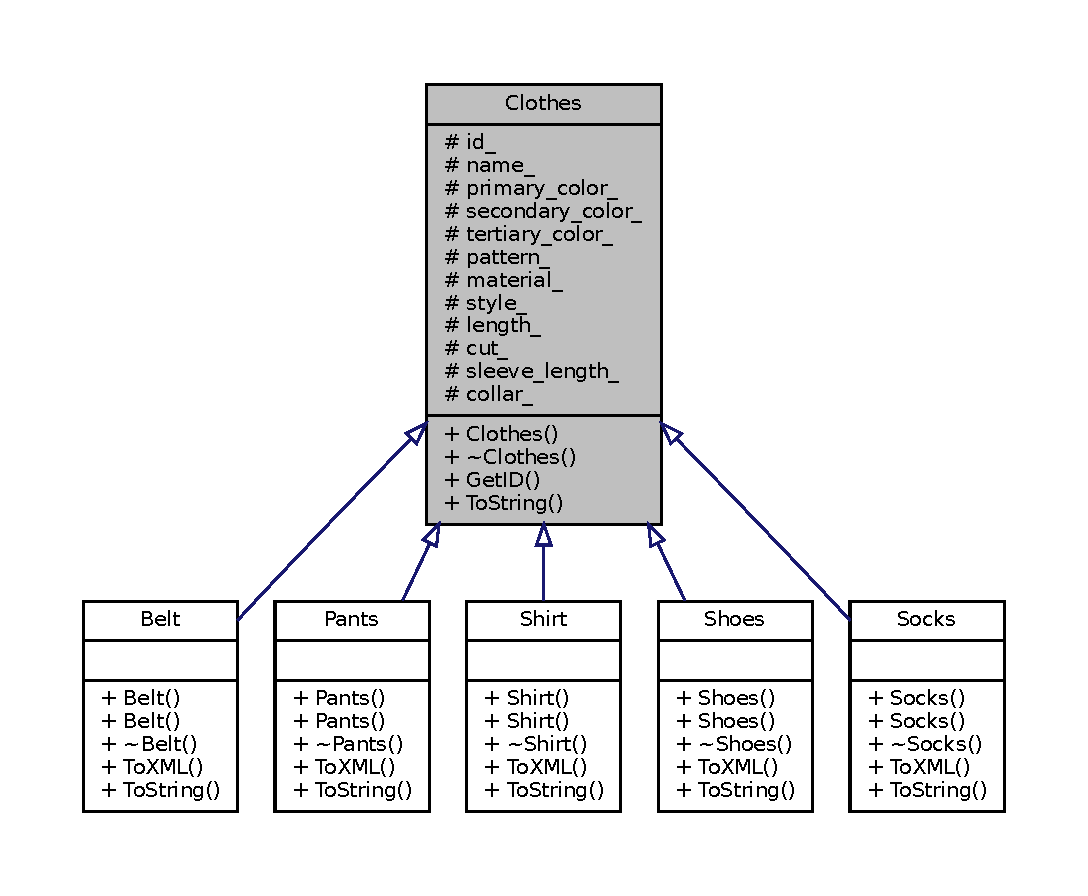
\includegraphics[width=350pt]{classClothes__inherit__graph}
\end{center}
\end{figure}


Collaboration diagram for Clothes\+:\nopagebreak
\begin{figure}[H]
\begin{center}
\leavevmode
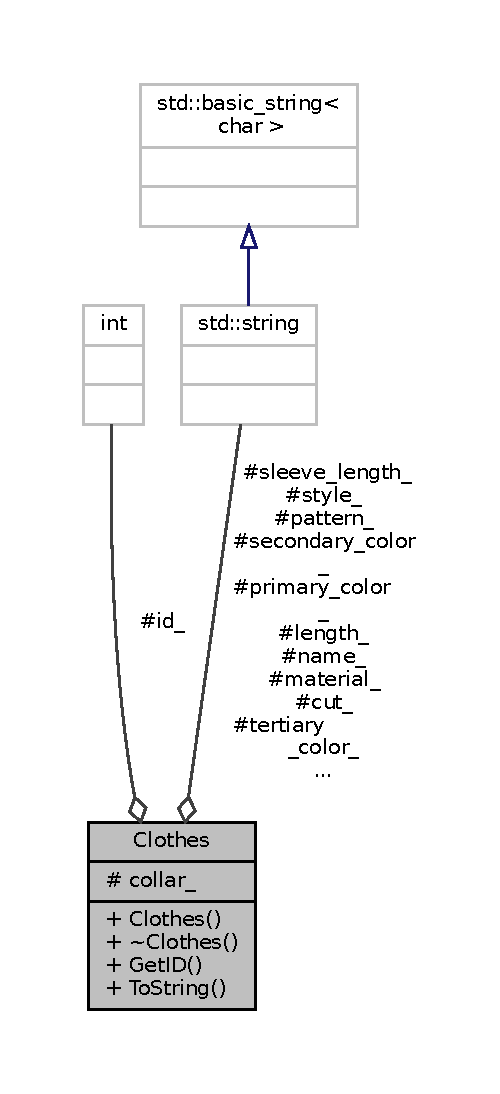
\includegraphics[width=240pt]{classClothes__coll__graph}
\end{center}
\end{figure}
\subsection*{Public Member Functions}
\begin{DoxyCompactItemize}
\item 
\mbox{\hyperlink{classClothes_a3df0bb45365fe4b9c82fde551207aa18}{Clothes}} ()
\item 
virtual \mbox{\hyperlink{classClothes_a90ab914d23c6870f19e387922f48fe88}{$\sim$\+Clothes}} ()
\item 
int \mbox{\hyperlink{classClothes_a3f6dac172f333126d19010f85ec44e4c}{Get\+ID}} ()
\item 
virtual string \mbox{\hyperlink{classClothes_a953d143394e9a2c007ab0c3a638973cf}{To\+String}} () const =0
\end{DoxyCompactItemize}
\subsection*{Protected Attributes}
\begin{DoxyCompactItemize}
\item 
int \mbox{\hyperlink{classClothes_a8978d931db5ca47c3ccea30def4ae83e}{id\+\_\+}} = \mbox{\hyperlink{clothes_8h_a77186917343a417a2369cdff0bc86d31}{k\+Dummy\+ID}}
\begin{DoxyCompactList}\small\item\em Global unique identifier. \end{DoxyCompactList}\item 
string \mbox{\hyperlink{classClothes_a7f2275aaae24224d60c48af922c31b65}{name\+\_\+}} = \mbox{\hyperlink{clothes_8h_adba739b5125fd5a4066ec0ef063c0657}{k\+Dummy\+Name}}
\begin{DoxyCompactList}\small\item\em User readable name. \end{DoxyCompactList}\item 
string \mbox{\hyperlink{classClothes_a7cb005bf6cbb7f4eaa40f1b31817559c}{primary\+\_\+color\+\_\+}} = \mbox{\hyperlink{clothes_8h_a1b9c685d3bf2811d95b65e0d396c1344}{k\+Dummy\+Prim\+Color}}
\begin{DoxyCompactList}\small\item\em Primary color. \end{DoxyCompactList}\item 
string \mbox{\hyperlink{classClothes_ab8f55f67b956b25d71260cffcf273673}{secondary\+\_\+color\+\_\+}} = \mbox{\hyperlink{clothes_8h_a71c39811135425d881af7760da63a73a}{k\+Dummy\+Sec\+Color}}
\begin{DoxyCompactList}\small\item\em Secondary color. \end{DoxyCompactList}\item 
string \mbox{\hyperlink{classClothes_a3c5f1e7ab531e3ba7a38b930da8078a0}{tertiary\+\_\+color\+\_\+}} = \mbox{\hyperlink{clothes_8h_a094dde85547895fd70dafb3ab10c6783}{k\+Dummy\+Tert\+Color}}
\begin{DoxyCompactList}\small\item\em Tertiary color. \end{DoxyCompactList}\item 
string \mbox{\hyperlink{classClothes_a1d40145a4eb6d28441f112f030ab5d35}{pattern\+\_\+}} = \mbox{\hyperlink{clothes_8h_a2e72ae4d77adb7bc9cbecf4dea1e9e22}{k\+Dummy\+Pattern}}
\begin{DoxyCompactList}\small\item\em Design pattern. \end{DoxyCompactList}\item 
string \mbox{\hyperlink{classClothes_adbb9ed311f14ccbb1e4fe0e8378a95d4}{material\+\_\+}} = \mbox{\hyperlink{clothes_8h_a9df1268c6668ae4e2a728ccf032cc33d}{k\+Dummy\+Material}}
\begin{DoxyCompactList}\small\item\em Material. \end{DoxyCompactList}\item 
string \mbox{\hyperlink{classClothes_aa85ed2b95110d8c477a1aca9cb403f98}{style\+\_\+}} = \mbox{\hyperlink{clothes_8h_a9deec6ed1f40928bfa0040eeab95ed6b}{k\+Dummy\+Style}}
\begin{DoxyCompactList}\small\item\em Design style. \end{DoxyCompactList}\item 
string \mbox{\hyperlink{classClothes_ae02603eda727e33caf46ec30e761e3c3}{length\+\_\+}} = \mbox{\hyperlink{clothes_8h_a1624256dcecfb0995a74c36142593770}{k\+Dummy\+Length}}
\begin{DoxyCompactList}\small\item\em Length of the clothing. \end{DoxyCompactList}\item 
string \mbox{\hyperlink{classClothes_ac1c2286c8928a5eee91d818a098a44ac}{cut\+\_\+}} = \mbox{\hyperlink{clothes_8h_a8a6eb066049b009439505355aeaae375}{k\+Dummy\+Cut}}
\begin{DoxyCompactList}\small\item\em Cut of the clothing. \end{DoxyCompactList}\item 
string \mbox{\hyperlink{classClothes_a012aeb71e62ebaf9b5b5dd700cc8d5db}{sleeve\+\_\+length\+\_\+}} = \mbox{\hyperlink{clothes_8h_a0f53dde6a2c4c344bb7da50655497350}{k\+Dummy\+Sleeve\+Length}}
\begin{DoxyCompactList}\small\item\em Length of the sleeve. \end{DoxyCompactList}\item 
string \mbox{\hyperlink{classClothes_ae2e5026257b3a2f2ddbf61757fd3b57b}{collar\+\_\+}} = \mbox{\hyperlink{clothes_8h_ac06c9f556f68bcd2829e36c55b70a86e}{k\+Dummy\+Collar}}
\begin{DoxyCompactList}\small\item\em Type of collar. \end{DoxyCompactList}\end{DoxyCompactItemize}


\subsection{Detailed Description}
\mbox{\hyperlink{classClothes}{Clothes}} abstract class to be used by members of closet. Handles the light work. 

\begin{DoxyAuthor}{Author}
Stephen M. Reaves 
\end{DoxyAuthor}
\begin{DoxyDate}{Date}
July 14th, 2018
\end{DoxyDate}
These global variables are set for all clothes, but not all clothes use them. For instance, pants will never need a \textquotesingle{}collar\textquotesingle{} variable, but they do to make inheritence easier 

\subsection{Constructor \& Destructor Documentation}
\mbox{\Hypertarget{classClothes_a3df0bb45365fe4b9c82fde551207aa18}\label{classClothes_a3df0bb45365fe4b9c82fde551207aa18}} 
\index{Clothes@{Clothes}!Clothes@{Clothes}}
\index{Clothes@{Clothes}!Clothes@{Clothes}}
\subsubsection{\texorpdfstring{Clothes()}{Clothes()}}
{\footnotesize\ttfamily Clothes\+::\+Clothes (\begin{DoxyParamCaption}{ }\end{DoxyParamCaption})\hspace{0.3cm}{\ttfamily [inline]}}

\mbox{\Hypertarget{classClothes_a90ab914d23c6870f19e387922f48fe88}\label{classClothes_a90ab914d23c6870f19e387922f48fe88}} 
\index{Clothes@{Clothes}!````~Clothes@{$\sim$\+Clothes}}
\index{````~Clothes@{$\sim$\+Clothes}!Clothes@{Clothes}}
\subsubsection{\texorpdfstring{$\sim$\+Clothes()}{~Clothes()}}
{\footnotesize\ttfamily virtual Clothes\+::$\sim$\+Clothes (\begin{DoxyParamCaption}{ }\end{DoxyParamCaption})\hspace{0.3cm}{\ttfamily [inline]}, {\ttfamily [virtual]}}



\subsection{Member Function Documentation}
\mbox{\Hypertarget{classClothes_a3f6dac172f333126d19010f85ec44e4c}\label{classClothes_a3f6dac172f333126d19010f85ec44e4c}} 
\index{Clothes@{Clothes}!Get\+ID@{Get\+ID}}
\index{Get\+ID@{Get\+ID}!Clothes@{Clothes}}
\subsubsection{\texorpdfstring{Get\+I\+D()}{GetID()}}
{\footnotesize\ttfamily int Clothes\+::\+Get\+ID (\begin{DoxyParamCaption}{ }\end{DoxyParamCaption})\hspace{0.3cm}{\ttfamily [inline]}}

Here is the caller graph for this function\+:
\nopagebreak
\begin{figure}[H]
\begin{center}
\leavevmode
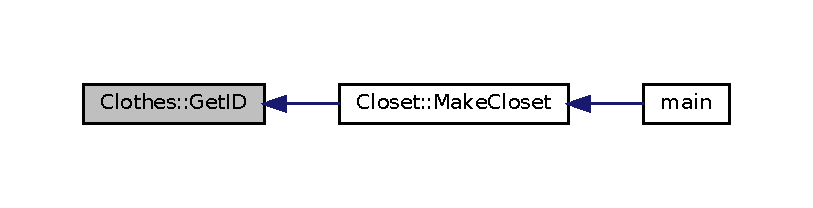
\includegraphics[width=350pt]{classClothes_a3f6dac172f333126d19010f85ec44e4c_icgraph}
\end{center}
\end{figure}
\mbox{\Hypertarget{classClothes_a953d143394e9a2c007ab0c3a638973cf}\label{classClothes_a953d143394e9a2c007ab0c3a638973cf}} 
\index{Clothes@{Clothes}!To\+String@{To\+String}}
\index{To\+String@{To\+String}!Clothes@{Clothes}}
\subsubsection{\texorpdfstring{To\+String()}{ToString()}}
{\footnotesize\ttfamily virtual string Clothes\+::\+To\+String (\begin{DoxyParamCaption}{ }\end{DoxyParamCaption}) const\hspace{0.3cm}{\ttfamily [pure virtual]}}

This is what makes this a purely abstract class. The implementation of these will be changed from one article of clothing to the next. 

Implemented in \mbox{\hyperlink{classShoes_a9b1bcc00ec7ef920d34bf9193c96a1ce}{Shoes}}, \mbox{\hyperlink{classSocks_aad237fbcc4ccf36a2956fcdef8760683}{Socks}}, \mbox{\hyperlink{classBelt_af09e2b5e51b7603ec5dede2e6b0a753f}{Belt}}, \mbox{\hyperlink{classPants_a9b5fcde766a77877bf428e18c65f1e70}{Pants}}, and \mbox{\hyperlink{classShirt_ab85aaa20a603d63f4144d1b42d9b616d}{Shirt}}.



\subsection{Member Data Documentation}
\mbox{\Hypertarget{classClothes_ae2e5026257b3a2f2ddbf61757fd3b57b}\label{classClothes_ae2e5026257b3a2f2ddbf61757fd3b57b}} 
\index{Clothes@{Clothes}!collar\+\_\+@{collar\+\_\+}}
\index{collar\+\_\+@{collar\+\_\+}!Clothes@{Clothes}}
\subsubsection{\texorpdfstring{collar\+\_\+}{collar\_}}
{\footnotesize\ttfamily string Clothes\+::collar\+\_\+ = \mbox{\hyperlink{clothes_8h_ac06c9f556f68bcd2829e36c55b70a86e}{k\+Dummy\+Collar}}\hspace{0.3cm}{\ttfamily [protected]}}



Type of collar. 

\mbox{\Hypertarget{classClothes_ac1c2286c8928a5eee91d818a098a44ac}\label{classClothes_ac1c2286c8928a5eee91d818a098a44ac}} 
\index{Clothes@{Clothes}!cut\+\_\+@{cut\+\_\+}}
\index{cut\+\_\+@{cut\+\_\+}!Clothes@{Clothes}}
\subsubsection{\texorpdfstring{cut\+\_\+}{cut\_}}
{\footnotesize\ttfamily string Clothes\+::cut\+\_\+ = \mbox{\hyperlink{clothes_8h_a8a6eb066049b009439505355aeaae375}{k\+Dummy\+Cut}}\hspace{0.3cm}{\ttfamily [protected]}}



Cut of the clothing. 

\mbox{\Hypertarget{classClothes_a8978d931db5ca47c3ccea30def4ae83e}\label{classClothes_a8978d931db5ca47c3ccea30def4ae83e}} 
\index{Clothes@{Clothes}!id\+\_\+@{id\+\_\+}}
\index{id\+\_\+@{id\+\_\+}!Clothes@{Clothes}}
\subsubsection{\texorpdfstring{id\+\_\+}{id\_}}
{\footnotesize\ttfamily int Clothes\+::id\+\_\+ = \mbox{\hyperlink{clothes_8h_a77186917343a417a2369cdff0bc86d31}{k\+Dummy\+ID}}\hspace{0.3cm}{\ttfamily [protected]}}



Global unique identifier. 

\mbox{\Hypertarget{classClothes_ae02603eda727e33caf46ec30e761e3c3}\label{classClothes_ae02603eda727e33caf46ec30e761e3c3}} 
\index{Clothes@{Clothes}!length\+\_\+@{length\+\_\+}}
\index{length\+\_\+@{length\+\_\+}!Clothes@{Clothes}}
\subsubsection{\texorpdfstring{length\+\_\+}{length\_}}
{\footnotesize\ttfamily string Clothes\+::length\+\_\+ = \mbox{\hyperlink{clothes_8h_a1624256dcecfb0995a74c36142593770}{k\+Dummy\+Length}}\hspace{0.3cm}{\ttfamily [protected]}}



Length of the clothing. 

\mbox{\Hypertarget{classClothes_adbb9ed311f14ccbb1e4fe0e8378a95d4}\label{classClothes_adbb9ed311f14ccbb1e4fe0e8378a95d4}} 
\index{Clothes@{Clothes}!material\+\_\+@{material\+\_\+}}
\index{material\+\_\+@{material\+\_\+}!Clothes@{Clothes}}
\subsubsection{\texorpdfstring{material\+\_\+}{material\_}}
{\footnotesize\ttfamily string Clothes\+::material\+\_\+ = \mbox{\hyperlink{clothes_8h_a9df1268c6668ae4e2a728ccf032cc33d}{k\+Dummy\+Material}}\hspace{0.3cm}{\ttfamily [protected]}}



Material. 

\mbox{\Hypertarget{classClothes_a7f2275aaae24224d60c48af922c31b65}\label{classClothes_a7f2275aaae24224d60c48af922c31b65}} 
\index{Clothes@{Clothes}!name\+\_\+@{name\+\_\+}}
\index{name\+\_\+@{name\+\_\+}!Clothes@{Clothes}}
\subsubsection{\texorpdfstring{name\+\_\+}{name\_}}
{\footnotesize\ttfamily string Clothes\+::name\+\_\+ = \mbox{\hyperlink{clothes_8h_adba739b5125fd5a4066ec0ef063c0657}{k\+Dummy\+Name}}\hspace{0.3cm}{\ttfamily [protected]}}



User readable name. 

\mbox{\Hypertarget{classClothes_a1d40145a4eb6d28441f112f030ab5d35}\label{classClothes_a1d40145a4eb6d28441f112f030ab5d35}} 
\index{Clothes@{Clothes}!pattern\+\_\+@{pattern\+\_\+}}
\index{pattern\+\_\+@{pattern\+\_\+}!Clothes@{Clothes}}
\subsubsection{\texorpdfstring{pattern\+\_\+}{pattern\_}}
{\footnotesize\ttfamily string Clothes\+::pattern\+\_\+ = \mbox{\hyperlink{clothes_8h_a2e72ae4d77adb7bc9cbecf4dea1e9e22}{k\+Dummy\+Pattern}}\hspace{0.3cm}{\ttfamily [protected]}}



Design pattern. 

\mbox{\Hypertarget{classClothes_a7cb005bf6cbb7f4eaa40f1b31817559c}\label{classClothes_a7cb005bf6cbb7f4eaa40f1b31817559c}} 
\index{Clothes@{Clothes}!primary\+\_\+color\+\_\+@{primary\+\_\+color\+\_\+}}
\index{primary\+\_\+color\+\_\+@{primary\+\_\+color\+\_\+}!Clothes@{Clothes}}
\subsubsection{\texorpdfstring{primary\+\_\+color\+\_\+}{primary\_color\_}}
{\footnotesize\ttfamily string Clothes\+::primary\+\_\+color\+\_\+ = \mbox{\hyperlink{clothes_8h_a1b9c685d3bf2811d95b65e0d396c1344}{k\+Dummy\+Prim\+Color}}\hspace{0.3cm}{\ttfamily [protected]}}



Primary color. 

\mbox{\Hypertarget{classClothes_ab8f55f67b956b25d71260cffcf273673}\label{classClothes_ab8f55f67b956b25d71260cffcf273673}} 
\index{Clothes@{Clothes}!secondary\+\_\+color\+\_\+@{secondary\+\_\+color\+\_\+}}
\index{secondary\+\_\+color\+\_\+@{secondary\+\_\+color\+\_\+}!Clothes@{Clothes}}
\subsubsection{\texorpdfstring{secondary\+\_\+color\+\_\+}{secondary\_color\_}}
{\footnotesize\ttfamily string Clothes\+::secondary\+\_\+color\+\_\+ = \mbox{\hyperlink{clothes_8h_a71c39811135425d881af7760da63a73a}{k\+Dummy\+Sec\+Color}}\hspace{0.3cm}{\ttfamily [protected]}}



Secondary color. 

\mbox{\Hypertarget{classClothes_a012aeb71e62ebaf9b5b5dd700cc8d5db}\label{classClothes_a012aeb71e62ebaf9b5b5dd700cc8d5db}} 
\index{Clothes@{Clothes}!sleeve\+\_\+length\+\_\+@{sleeve\+\_\+length\+\_\+}}
\index{sleeve\+\_\+length\+\_\+@{sleeve\+\_\+length\+\_\+}!Clothes@{Clothes}}
\subsubsection{\texorpdfstring{sleeve\+\_\+length\+\_\+}{sleeve\_length\_}}
{\footnotesize\ttfamily string Clothes\+::sleeve\+\_\+length\+\_\+ = \mbox{\hyperlink{clothes_8h_a0f53dde6a2c4c344bb7da50655497350}{k\+Dummy\+Sleeve\+Length}}\hspace{0.3cm}{\ttfamily [protected]}}



Length of the sleeve. 

\mbox{\Hypertarget{classClothes_aa85ed2b95110d8c477a1aca9cb403f98}\label{classClothes_aa85ed2b95110d8c477a1aca9cb403f98}} 
\index{Clothes@{Clothes}!style\+\_\+@{style\+\_\+}}
\index{style\+\_\+@{style\+\_\+}!Clothes@{Clothes}}
\subsubsection{\texorpdfstring{style\+\_\+}{style\_}}
{\footnotesize\ttfamily string Clothes\+::style\+\_\+ = \mbox{\hyperlink{clothes_8h_a9deec6ed1f40928bfa0040eeab95ed6b}{k\+Dummy\+Style}}\hspace{0.3cm}{\ttfamily [protected]}}



Design style. 

\mbox{\Hypertarget{classClothes_a3c5f1e7ab531e3ba7a38b930da8078a0}\label{classClothes_a3c5f1e7ab531e3ba7a38b930da8078a0}} 
\index{Clothes@{Clothes}!tertiary\+\_\+color\+\_\+@{tertiary\+\_\+color\+\_\+}}
\index{tertiary\+\_\+color\+\_\+@{tertiary\+\_\+color\+\_\+}!Clothes@{Clothes}}
\subsubsection{\texorpdfstring{tertiary\+\_\+color\+\_\+}{tertiary\_color\_}}
{\footnotesize\ttfamily string Clothes\+::tertiary\+\_\+color\+\_\+ = \mbox{\hyperlink{clothes_8h_a094dde85547895fd70dafb3ab10c6783}{k\+Dummy\+Tert\+Color}}\hspace{0.3cm}{\ttfamily [protected]}}



Tertiary color. 



The documentation for this class was generated from the following file\+:\begin{DoxyCompactItemize}
\item 
\mbox{\hyperlink{clothes_8h}{clothes.\+h}}\end{DoxyCompactItemize}

\hypertarget{classNcurses}{}\section{Ncurses Class Reference}
\label{classNcurses}\index{Ncurses@{Ncurses}}


{\ttfamily \#include $<$ncurses.\+h$>$}



Collaboration diagram for Ncurses\+:\nopagebreak
\begin{figure}[H]
\begin{center}
\leavevmode
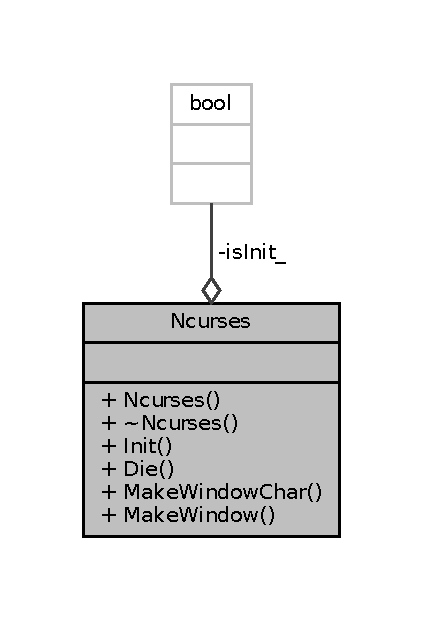
\includegraphics[width=203pt]{classNcurses__coll__graph}
\end{center}
\end{figure}
\subsection*{Public Member Functions}
\begin{DoxyCompactItemize}
\item 
\mbox{\hyperlink{classNcurses_a2565bd187834633fd68b595184ee2acf}{Ncurses}} ()
\item 
virtual \mbox{\hyperlink{classNcurses_a4197da9eb0dafba570c2f60a6ce0124e}{$\sim$\+Ncurses}} ()
\item 
bool \mbox{\hyperlink{classNcurses_a9966b2b23b522e415232976acfa1d18f}{Init}} ()
\item 
void \mbox{\hyperlink{classNcurses_af9467a004e66043d4dbe540e24524f1f}{Die}} ()
\item 
char \mbox{\hyperlink{classNcurses_a2b4916627ad802a840b95cf65766773f}{Make\+Window\+Char}} (string message)
\item 
string \mbox{\hyperlink{classNcurses_a1d8def11419a444c5696b5043da680d4}{Make\+Window}} (string message)
\end{DoxyCompactItemize}
\subsection*{Private Attributes}
\begin{DoxyCompactItemize}
\item 
bool \mbox{\hyperlink{classNcurses_adce6b18f601709b3843fb36fa7b91764}{is\+Init\+\_\+}} = false
\end{DoxyCompactItemize}


\subsection{Constructor \& Destructor Documentation}
\mbox{\Hypertarget{classNcurses_a2565bd187834633fd68b595184ee2acf}\label{classNcurses_a2565bd187834633fd68b595184ee2acf}} 
\index{Ncurses@{Ncurses}!Ncurses@{Ncurses}}
\index{Ncurses@{Ncurses}!Ncurses@{Ncurses}}
\subsubsection{\texorpdfstring{Ncurses()}{Ncurses()}}
{\footnotesize\ttfamily Ncurses\+::\+Ncurses (\begin{DoxyParamCaption}{ }\end{DoxyParamCaption})}

\mbox{\Hypertarget{classNcurses_a4197da9eb0dafba570c2f60a6ce0124e}\label{classNcurses_a4197da9eb0dafba570c2f60a6ce0124e}} 
\index{Ncurses@{Ncurses}!````~Ncurses@{$\sim$\+Ncurses}}
\index{````~Ncurses@{$\sim$\+Ncurses}!Ncurses@{Ncurses}}
\subsubsection{\texorpdfstring{$\sim$\+Ncurses()}{~Ncurses()}}
{\footnotesize\ttfamily Ncurses\+::$\sim$\+Ncurses (\begin{DoxyParamCaption}{ }\end{DoxyParamCaption})\hspace{0.3cm}{\ttfamily [virtual]}}



\subsection{Member Function Documentation}
\mbox{\Hypertarget{classNcurses_af9467a004e66043d4dbe540e24524f1f}\label{classNcurses_af9467a004e66043d4dbe540e24524f1f}} 
\index{Ncurses@{Ncurses}!Die@{Die}}
\index{Die@{Die}!Ncurses@{Ncurses}}
\subsubsection{\texorpdfstring{Die()}{Die()}}
{\footnotesize\ttfamily void Ncurses\+::\+Die (\begin{DoxyParamCaption}{ }\end{DoxyParamCaption})}

Here is the caller graph for this function\+:\nopagebreak
\begin{figure}[H]
\begin{center}
\leavevmode
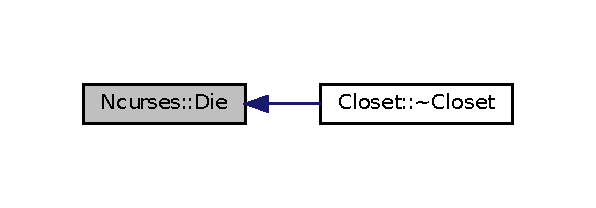
\includegraphics[width=286pt]{classNcurses_af9467a004e66043d4dbe540e24524f1f_icgraph}
\end{center}
\end{figure}
\mbox{\Hypertarget{classNcurses_a9966b2b23b522e415232976acfa1d18f}\label{classNcurses_a9966b2b23b522e415232976acfa1d18f}} 
\index{Ncurses@{Ncurses}!Init@{Init}}
\index{Init@{Init}!Ncurses@{Ncurses}}
\subsubsection{\texorpdfstring{Init()}{Init()}}
{\footnotesize\ttfamily bool Ncurses\+::\+Init (\begin{DoxyParamCaption}{ }\end{DoxyParamCaption})}

Here is the caller graph for this function\+:\nopagebreak
\begin{figure}[H]
\begin{center}
\leavevmode
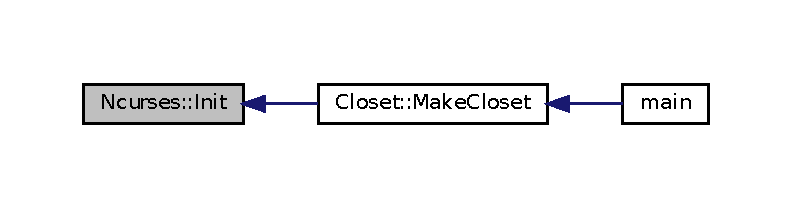
\includegraphics[width=350pt]{classNcurses_a9966b2b23b522e415232976acfa1d18f_icgraph}
\end{center}
\end{figure}
\mbox{\Hypertarget{classNcurses_a1d8def11419a444c5696b5043da680d4}\label{classNcurses_a1d8def11419a444c5696b5043da680d4}} 
\index{Ncurses@{Ncurses}!Make\+Window@{Make\+Window}}
\index{Make\+Window@{Make\+Window}!Ncurses@{Ncurses}}
\subsubsection{\texorpdfstring{Make\+Window()}{MakeWindow()}}
{\footnotesize\ttfamily string Ncurses\+::\+Make\+Window (\begin{DoxyParamCaption}\item[{string}]{message }\end{DoxyParamCaption})}

Here is the caller graph for this function\+:\nopagebreak
\begin{figure}[H]
\begin{center}
\leavevmode
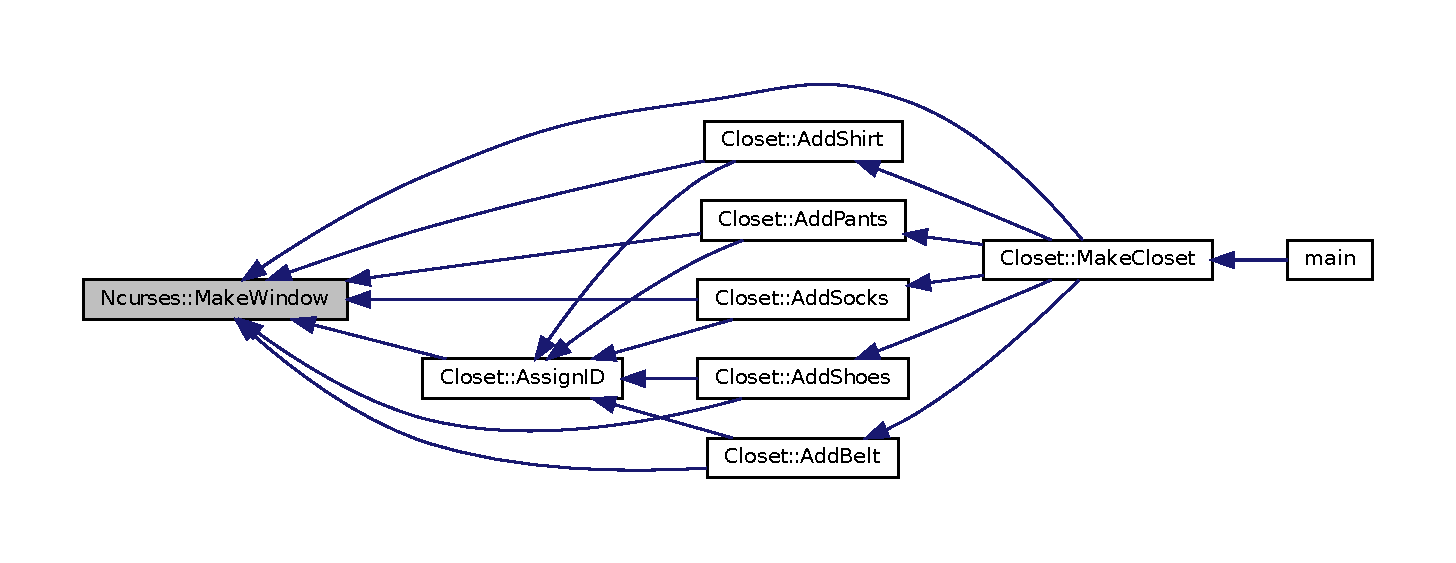
\includegraphics[width=350pt]{classNcurses_a1d8def11419a444c5696b5043da680d4_icgraph}
\end{center}
\end{figure}
\mbox{\Hypertarget{classNcurses_a2b4916627ad802a840b95cf65766773f}\label{classNcurses_a2b4916627ad802a840b95cf65766773f}} 
\index{Ncurses@{Ncurses}!Make\+Window\+Char@{Make\+Window\+Char}}
\index{Make\+Window\+Char@{Make\+Window\+Char}!Ncurses@{Ncurses}}
\subsubsection{\texorpdfstring{Make\+Window\+Char()}{MakeWindowChar()}}
{\footnotesize\ttfamily char Ncurses\+::\+Make\+Window\+Char (\begin{DoxyParamCaption}\item[{string}]{message }\end{DoxyParamCaption})}

Here is the caller graph for this function\+:\nopagebreak
\begin{figure}[H]
\begin{center}
\leavevmode
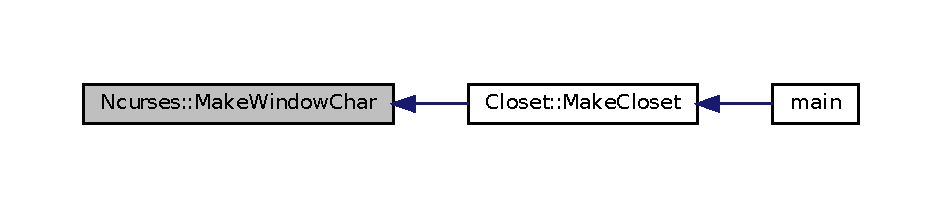
\includegraphics[width=350pt]{classNcurses_a2b4916627ad802a840b95cf65766773f_icgraph}
\end{center}
\end{figure}


\subsection{Member Data Documentation}
\mbox{\Hypertarget{classNcurses_adce6b18f601709b3843fb36fa7b91764}\label{classNcurses_adce6b18f601709b3843fb36fa7b91764}} 
\index{Ncurses@{Ncurses}!is\+Init\+\_\+@{is\+Init\+\_\+}}
\index{is\+Init\+\_\+@{is\+Init\+\_\+}!Ncurses@{Ncurses}}
\subsubsection{\texorpdfstring{is\+Init\+\_\+}{isInit\_}}
{\footnotesize\ttfamily bool Ncurses\+::is\+Init\+\_\+ = false\hspace{0.3cm}{\ttfamily [private]}}



The documentation for this class was generated from the following files\+:\begin{DoxyCompactItemize}
\item 
\mbox{\hyperlink{ncurses_8h}{ncurses.\+h}}\item 
\mbox{\hyperlink{ncurses_8cc}{ncurses.\+cc}}\end{DoxyCompactItemize}

\hypertarget{classPants}{}\section{Pants Class Reference}
\label{classPants}\index{Pants@{Pants}}


{\ttfamily \#include $<$pants.\+h$>$}



Inheritance diagram for Pants\+:\nopagebreak
\begin{figure}[H]
\begin{center}
\leavevmode
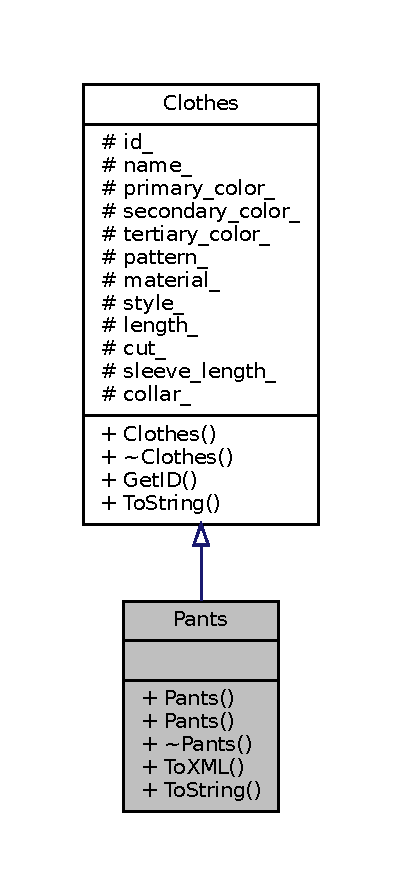
\includegraphics[width=193pt]{classPants__inherit__graph}
\end{center}
\end{figure}


Collaboration diagram for Pants\+:\nopagebreak
\begin{figure}[H]
\begin{center}
\leavevmode
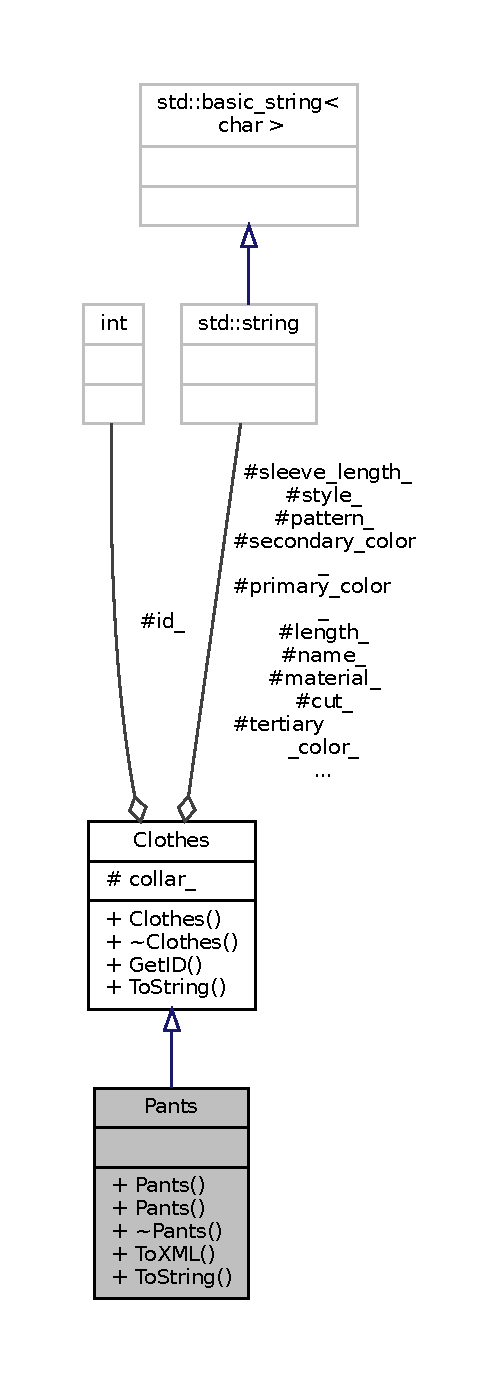
\includegraphics[height=550pt]{classPants__coll__graph}
\end{center}
\end{figure}
\subsection*{Public Member Functions}
\begin{DoxyCompactItemize}
\item 
\mbox{\hyperlink{classPants_a6e19084b693fdb83029addacdecdc2e2}{Pants}} ()
\item 
\mbox{\hyperlink{classPants_a9ca6f6ddce0ac46556b6e56a9d73ddd0}{Pants}} (int id, string name, string prim\+\_\+color, string sec\+\_\+color, string tert\+\_\+color, string material, string length, string cut)
\item 
virtual \mbox{\hyperlink{classPants_a22fa728c533ab55fbbd1b77b8d9ad860}{$\sim$\+Pants}} ()
\item 
string \mbox{\hyperlink{classPants_aa62270b70cbb40b7b420f1091ad7e43b}{To\+X\+ML}} () const
\item 
string \mbox{\hyperlink{classPants_a9b5fcde766a77877bf428e18c65f1e70}{To\+String}} () const
\item 
int \mbox{\hyperlink{classClothes_a3f6dac172f333126d19010f85ec44e4c}{Get\+ID}} ()
\end{DoxyCompactItemize}
\subsection*{Protected Attributes}
\begin{DoxyCompactItemize}
\item 
int \mbox{\hyperlink{classClothes_a8978d931db5ca47c3ccea30def4ae83e}{id\+\_\+}} = \mbox{\hyperlink{clothes_8h_a77186917343a417a2369cdff0bc86d31}{k\+Dummy\+ID}}
\begin{DoxyCompactList}\small\item\em Global unique identifier. \end{DoxyCompactList}\item 
string \mbox{\hyperlink{classClothes_a7f2275aaae24224d60c48af922c31b65}{name\+\_\+}} = \mbox{\hyperlink{clothes_8h_adba739b5125fd5a4066ec0ef063c0657}{k\+Dummy\+Name}}
\begin{DoxyCompactList}\small\item\em User readable name. \end{DoxyCompactList}\item 
string \mbox{\hyperlink{classClothes_a7cb005bf6cbb7f4eaa40f1b31817559c}{primary\+\_\+color\+\_\+}} = \mbox{\hyperlink{clothes_8h_a1b9c685d3bf2811d95b65e0d396c1344}{k\+Dummy\+Prim\+Color}}
\begin{DoxyCompactList}\small\item\em Primary color. \end{DoxyCompactList}\item 
string \mbox{\hyperlink{classClothes_ab8f55f67b956b25d71260cffcf273673}{secondary\+\_\+color\+\_\+}} = \mbox{\hyperlink{clothes_8h_a71c39811135425d881af7760da63a73a}{k\+Dummy\+Sec\+Color}}
\begin{DoxyCompactList}\small\item\em Secondary color. \end{DoxyCompactList}\item 
string \mbox{\hyperlink{classClothes_a3c5f1e7ab531e3ba7a38b930da8078a0}{tertiary\+\_\+color\+\_\+}} = \mbox{\hyperlink{clothes_8h_a094dde85547895fd70dafb3ab10c6783}{k\+Dummy\+Tert\+Color}}
\begin{DoxyCompactList}\small\item\em Tertiary color. \end{DoxyCompactList}\item 
string \mbox{\hyperlink{classClothes_a1d40145a4eb6d28441f112f030ab5d35}{pattern\+\_\+}} = \mbox{\hyperlink{clothes_8h_a2e72ae4d77adb7bc9cbecf4dea1e9e22}{k\+Dummy\+Pattern}}
\begin{DoxyCompactList}\small\item\em Design pattern. \end{DoxyCompactList}\item 
string \mbox{\hyperlink{classClothes_adbb9ed311f14ccbb1e4fe0e8378a95d4}{material\+\_\+}} = \mbox{\hyperlink{clothes_8h_a9df1268c6668ae4e2a728ccf032cc33d}{k\+Dummy\+Material}}
\begin{DoxyCompactList}\small\item\em Material. \end{DoxyCompactList}\item 
string \mbox{\hyperlink{classClothes_aa85ed2b95110d8c477a1aca9cb403f98}{style\+\_\+}} = \mbox{\hyperlink{clothes_8h_a9deec6ed1f40928bfa0040eeab95ed6b}{k\+Dummy\+Style}}
\begin{DoxyCompactList}\small\item\em Design style. \end{DoxyCompactList}\item 
string \mbox{\hyperlink{classClothes_ae02603eda727e33caf46ec30e761e3c3}{length\+\_\+}} = \mbox{\hyperlink{clothes_8h_a1624256dcecfb0995a74c36142593770}{k\+Dummy\+Length}}
\begin{DoxyCompactList}\small\item\em Length of the clothing. \end{DoxyCompactList}\item 
string \mbox{\hyperlink{classClothes_ac1c2286c8928a5eee91d818a098a44ac}{cut\+\_\+}} = \mbox{\hyperlink{clothes_8h_a8a6eb066049b009439505355aeaae375}{k\+Dummy\+Cut}}
\begin{DoxyCompactList}\small\item\em Cut of the clothing. \end{DoxyCompactList}\item 
string \mbox{\hyperlink{classClothes_a012aeb71e62ebaf9b5b5dd700cc8d5db}{sleeve\+\_\+length\+\_\+}} = \mbox{\hyperlink{clothes_8h_a0f53dde6a2c4c344bb7da50655497350}{k\+Dummy\+Sleeve\+Length}}
\begin{DoxyCompactList}\small\item\em Length of the sleeve. \end{DoxyCompactList}\item 
string \mbox{\hyperlink{classClothes_ae2e5026257b3a2f2ddbf61757fd3b57b}{collar\+\_\+}} = \mbox{\hyperlink{clothes_8h_ac06c9f556f68bcd2829e36c55b70a86e}{k\+Dummy\+Collar}}
\begin{DoxyCompactList}\small\item\em Type of collar. \end{DoxyCompactList}\end{DoxyCompactItemize}


\subsection{Constructor \& Destructor Documentation}
\mbox{\Hypertarget{classPants_a6e19084b693fdb83029addacdecdc2e2}\label{classPants_a6e19084b693fdb83029addacdecdc2e2}} 
\index{Pants@{Pants}!Pants@{Pants}}
\index{Pants@{Pants}!Pants@{Pants}}
\subsubsection{\texorpdfstring{Pants()}{Pants()}\hspace{0.1cm}{\footnotesize\ttfamily [1/2]}}
{\footnotesize\ttfamily Pants\+::\+Pants (\begin{DoxyParamCaption}{ }\end{DoxyParamCaption})}

\mbox{\Hypertarget{classPants_a9ca6f6ddce0ac46556b6e56a9d73ddd0}\label{classPants_a9ca6f6ddce0ac46556b6e56a9d73ddd0}} 
\index{Pants@{Pants}!Pants@{Pants}}
\index{Pants@{Pants}!Pants@{Pants}}
\subsubsection{\texorpdfstring{Pants()}{Pants()}\hspace{0.1cm}{\footnotesize\ttfamily [2/2]}}
{\footnotesize\ttfamily Pants\+::\+Pants (\begin{DoxyParamCaption}\item[{int}]{id,  }\item[{string}]{name,  }\item[{string}]{prim\+\_\+color,  }\item[{string}]{sec\+\_\+color,  }\item[{string}]{tert\+\_\+color,  }\item[{string}]{material,  }\item[{string}]{length,  }\item[{string}]{cut }\end{DoxyParamCaption})}



References \mbox{\hyperlink{classClothes_ac1c2286c8928a5eee91d818a098a44ac}{Clothes\+::cut\+\_\+}}, \mbox{\hyperlink{classClothes_a8978d931db5ca47c3ccea30def4ae83e}{Clothes\+::id\+\_\+}}, \mbox{\hyperlink{classClothes_ae02603eda727e33caf46ec30e761e3c3}{Clothes\+::length\+\_\+}}, \mbox{\hyperlink{classClothes_adbb9ed311f14ccbb1e4fe0e8378a95d4}{Clothes\+::material\+\_\+}}, \mbox{\hyperlink{classClothes_a7f2275aaae24224d60c48af922c31b65}{Clothes\+::name\+\_\+}}, \mbox{\hyperlink{classClothes_a7cb005bf6cbb7f4eaa40f1b31817559c}{Clothes\+::primary\+\_\+color\+\_\+}}, \mbox{\hyperlink{classClothes_ab8f55f67b956b25d71260cffcf273673}{Clothes\+::secondary\+\_\+color\+\_\+}}, and \mbox{\hyperlink{classClothes_a3c5f1e7ab531e3ba7a38b930da8078a0}{Clothes\+::tertiary\+\_\+color\+\_\+}}.

\mbox{\Hypertarget{classPants_a22fa728c533ab55fbbd1b77b8d9ad860}\label{classPants_a22fa728c533ab55fbbd1b77b8d9ad860}} 
\index{Pants@{Pants}!````~Pants@{$\sim$\+Pants}}
\index{````~Pants@{$\sim$\+Pants}!Pants@{Pants}}
\subsubsection{\texorpdfstring{$\sim$\+Pants()}{~Pants()}}
{\footnotesize\ttfamily Pants\+::$\sim$\+Pants (\begin{DoxyParamCaption}{ }\end{DoxyParamCaption})\hspace{0.3cm}{\ttfamily [virtual]}}



\subsection{Member Function Documentation}
\mbox{\Hypertarget{classClothes_a3f6dac172f333126d19010f85ec44e4c}\label{classClothes_a3f6dac172f333126d19010f85ec44e4c}} 
\index{Pants@{Pants}!Get\+ID@{Get\+ID}}
\index{Get\+ID@{Get\+ID}!Pants@{Pants}}
\subsubsection{\texorpdfstring{Get\+I\+D()}{GetID()}}
{\footnotesize\ttfamily int Clothes\+::\+Get\+ID (\begin{DoxyParamCaption}{ }\end{DoxyParamCaption})\hspace{0.3cm}{\ttfamily [inline]}, {\ttfamily [inherited]}}

Here is the caller graph for this function\+:
\nopagebreak
\begin{figure}[H]
\begin{center}
\leavevmode
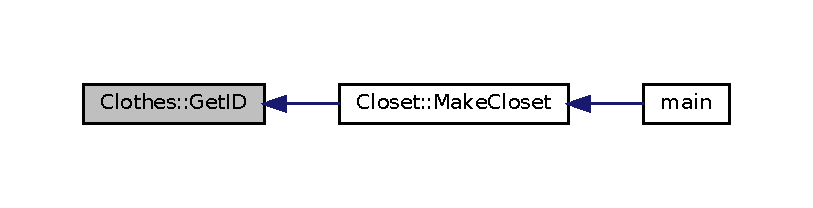
\includegraphics[width=350pt]{classClothes_a3f6dac172f333126d19010f85ec44e4c_icgraph}
\end{center}
\end{figure}
\mbox{\Hypertarget{classPants_a9b5fcde766a77877bf428e18c65f1e70}\label{classPants_a9b5fcde766a77877bf428e18c65f1e70}} 
\index{Pants@{Pants}!To\+String@{To\+String}}
\index{To\+String@{To\+String}!Pants@{Pants}}
\subsubsection{\texorpdfstring{To\+String()}{ToString()}}
{\footnotesize\ttfamily string Pants\+::\+To\+String (\begin{DoxyParamCaption}{ }\end{DoxyParamCaption}) const\hspace{0.3cm}{\ttfamily [virtual]}}

This is what makes this a purely abstract class. The implementation of these will be changed from one article of clothing to the next. 

Implements \mbox{\hyperlink{classClothes_a953d143394e9a2c007ab0c3a638973cf}{Clothes}}.



References \mbox{\hyperlink{classClothes_a8978d931db5ca47c3ccea30def4ae83e}{Clothes\+::id\+\_\+}}, \mbox{\hyperlink{classClothes_ae02603eda727e33caf46ec30e761e3c3}{Clothes\+::length\+\_\+}}, \mbox{\hyperlink{classClothes_adbb9ed311f14ccbb1e4fe0e8378a95d4}{Clothes\+::material\+\_\+}}, \mbox{\hyperlink{classClothes_a7f2275aaae24224d60c48af922c31b65}{Clothes\+::name\+\_\+}}, \mbox{\hyperlink{classClothes_a7cb005bf6cbb7f4eaa40f1b31817559c}{Clothes\+::primary\+\_\+color\+\_\+}}, \mbox{\hyperlink{classClothes_ab8f55f67b956b25d71260cffcf273673}{Clothes\+::secondary\+\_\+color\+\_\+}}, and \mbox{\hyperlink{classClothes_a3c5f1e7ab531e3ba7a38b930da8078a0}{Clothes\+::tertiary\+\_\+color\+\_\+}}.

\mbox{\Hypertarget{classPants_aa62270b70cbb40b7b420f1091ad7e43b}\label{classPants_aa62270b70cbb40b7b420f1091ad7e43b}} 
\index{Pants@{Pants}!To\+X\+ML@{To\+X\+ML}}
\index{To\+X\+ML@{To\+X\+ML}!Pants@{Pants}}
\subsubsection{\texorpdfstring{To\+X\+M\+L()}{ToXML()}}
{\footnotesize\ttfamily string Pants\+::\+To\+X\+ML (\begin{DoxyParamCaption}{ }\end{DoxyParamCaption}) const}



References \mbox{\hyperlink{classClothes_a8978d931db5ca47c3ccea30def4ae83e}{Clothes\+::id\+\_\+}}, \mbox{\hyperlink{classClothes_ae02603eda727e33caf46ec30e761e3c3}{Clothes\+::length\+\_\+}}, \mbox{\hyperlink{classClothes_adbb9ed311f14ccbb1e4fe0e8378a95d4}{Clothes\+::material\+\_\+}}, \mbox{\hyperlink{classClothes_a7f2275aaae24224d60c48af922c31b65}{Clothes\+::name\+\_\+}}, \mbox{\hyperlink{classClothes_a7cb005bf6cbb7f4eaa40f1b31817559c}{Clothes\+::primary\+\_\+color\+\_\+}}, \mbox{\hyperlink{classClothes_ab8f55f67b956b25d71260cffcf273673}{Clothes\+::secondary\+\_\+color\+\_\+}}, and \mbox{\hyperlink{classClothes_a3c5f1e7ab531e3ba7a38b930da8078a0}{Clothes\+::tertiary\+\_\+color\+\_\+}}.



\subsection{Member Data Documentation}
\mbox{\Hypertarget{classClothes_ae2e5026257b3a2f2ddbf61757fd3b57b}\label{classClothes_ae2e5026257b3a2f2ddbf61757fd3b57b}} 
\index{Pants@{Pants}!collar\+\_\+@{collar\+\_\+}}
\index{collar\+\_\+@{collar\+\_\+}!Pants@{Pants}}
\subsubsection{\texorpdfstring{collar\+\_\+}{collar\_}}
{\footnotesize\ttfamily string Clothes\+::collar\+\_\+ = \mbox{\hyperlink{clothes_8h_ac06c9f556f68bcd2829e36c55b70a86e}{k\+Dummy\+Collar}}\hspace{0.3cm}{\ttfamily [protected]}, {\ttfamily [inherited]}}



Type of collar. 

\mbox{\Hypertarget{classClothes_ac1c2286c8928a5eee91d818a098a44ac}\label{classClothes_ac1c2286c8928a5eee91d818a098a44ac}} 
\index{Pants@{Pants}!cut\+\_\+@{cut\+\_\+}}
\index{cut\+\_\+@{cut\+\_\+}!Pants@{Pants}}
\subsubsection{\texorpdfstring{cut\+\_\+}{cut\_}}
{\footnotesize\ttfamily string Clothes\+::cut\+\_\+ = \mbox{\hyperlink{clothes_8h_a8a6eb066049b009439505355aeaae375}{k\+Dummy\+Cut}}\hspace{0.3cm}{\ttfamily [protected]}, {\ttfamily [inherited]}}



Cut of the clothing. 

\mbox{\Hypertarget{classClothes_a8978d931db5ca47c3ccea30def4ae83e}\label{classClothes_a8978d931db5ca47c3ccea30def4ae83e}} 
\index{Pants@{Pants}!id\+\_\+@{id\+\_\+}}
\index{id\+\_\+@{id\+\_\+}!Pants@{Pants}}
\subsubsection{\texorpdfstring{id\+\_\+}{id\_}}
{\footnotesize\ttfamily int Clothes\+::id\+\_\+ = \mbox{\hyperlink{clothes_8h_a77186917343a417a2369cdff0bc86d31}{k\+Dummy\+ID}}\hspace{0.3cm}{\ttfamily [protected]}, {\ttfamily [inherited]}}



Global unique identifier. 

\mbox{\Hypertarget{classClothes_ae02603eda727e33caf46ec30e761e3c3}\label{classClothes_ae02603eda727e33caf46ec30e761e3c3}} 
\index{Pants@{Pants}!length\+\_\+@{length\+\_\+}}
\index{length\+\_\+@{length\+\_\+}!Pants@{Pants}}
\subsubsection{\texorpdfstring{length\+\_\+}{length\_}}
{\footnotesize\ttfamily string Clothes\+::length\+\_\+ = \mbox{\hyperlink{clothes_8h_a1624256dcecfb0995a74c36142593770}{k\+Dummy\+Length}}\hspace{0.3cm}{\ttfamily [protected]}, {\ttfamily [inherited]}}



Length of the clothing. 

\mbox{\Hypertarget{classClothes_adbb9ed311f14ccbb1e4fe0e8378a95d4}\label{classClothes_adbb9ed311f14ccbb1e4fe0e8378a95d4}} 
\index{Pants@{Pants}!material\+\_\+@{material\+\_\+}}
\index{material\+\_\+@{material\+\_\+}!Pants@{Pants}}
\subsubsection{\texorpdfstring{material\+\_\+}{material\_}}
{\footnotesize\ttfamily string Clothes\+::material\+\_\+ = \mbox{\hyperlink{clothes_8h_a9df1268c6668ae4e2a728ccf032cc33d}{k\+Dummy\+Material}}\hspace{0.3cm}{\ttfamily [protected]}, {\ttfamily [inherited]}}



Material. 

\mbox{\Hypertarget{classClothes_a7f2275aaae24224d60c48af922c31b65}\label{classClothes_a7f2275aaae24224d60c48af922c31b65}} 
\index{Pants@{Pants}!name\+\_\+@{name\+\_\+}}
\index{name\+\_\+@{name\+\_\+}!Pants@{Pants}}
\subsubsection{\texorpdfstring{name\+\_\+}{name\_}}
{\footnotesize\ttfamily string Clothes\+::name\+\_\+ = \mbox{\hyperlink{clothes_8h_adba739b5125fd5a4066ec0ef063c0657}{k\+Dummy\+Name}}\hspace{0.3cm}{\ttfamily [protected]}, {\ttfamily [inherited]}}



User readable name. 

\mbox{\Hypertarget{classClothes_a1d40145a4eb6d28441f112f030ab5d35}\label{classClothes_a1d40145a4eb6d28441f112f030ab5d35}} 
\index{Pants@{Pants}!pattern\+\_\+@{pattern\+\_\+}}
\index{pattern\+\_\+@{pattern\+\_\+}!Pants@{Pants}}
\subsubsection{\texorpdfstring{pattern\+\_\+}{pattern\_}}
{\footnotesize\ttfamily string Clothes\+::pattern\+\_\+ = \mbox{\hyperlink{clothes_8h_a2e72ae4d77adb7bc9cbecf4dea1e9e22}{k\+Dummy\+Pattern}}\hspace{0.3cm}{\ttfamily [protected]}, {\ttfamily [inherited]}}



Design pattern. 

\mbox{\Hypertarget{classClothes_a7cb005bf6cbb7f4eaa40f1b31817559c}\label{classClothes_a7cb005bf6cbb7f4eaa40f1b31817559c}} 
\index{Pants@{Pants}!primary\+\_\+color\+\_\+@{primary\+\_\+color\+\_\+}}
\index{primary\+\_\+color\+\_\+@{primary\+\_\+color\+\_\+}!Pants@{Pants}}
\subsubsection{\texorpdfstring{primary\+\_\+color\+\_\+}{primary\_color\_}}
{\footnotesize\ttfamily string Clothes\+::primary\+\_\+color\+\_\+ = \mbox{\hyperlink{clothes_8h_a1b9c685d3bf2811d95b65e0d396c1344}{k\+Dummy\+Prim\+Color}}\hspace{0.3cm}{\ttfamily [protected]}, {\ttfamily [inherited]}}



Primary color. 

\mbox{\Hypertarget{classClothes_ab8f55f67b956b25d71260cffcf273673}\label{classClothes_ab8f55f67b956b25d71260cffcf273673}} 
\index{Pants@{Pants}!secondary\+\_\+color\+\_\+@{secondary\+\_\+color\+\_\+}}
\index{secondary\+\_\+color\+\_\+@{secondary\+\_\+color\+\_\+}!Pants@{Pants}}
\subsubsection{\texorpdfstring{secondary\+\_\+color\+\_\+}{secondary\_color\_}}
{\footnotesize\ttfamily string Clothes\+::secondary\+\_\+color\+\_\+ = \mbox{\hyperlink{clothes_8h_a71c39811135425d881af7760da63a73a}{k\+Dummy\+Sec\+Color}}\hspace{0.3cm}{\ttfamily [protected]}, {\ttfamily [inherited]}}



Secondary color. 

\mbox{\Hypertarget{classClothes_a012aeb71e62ebaf9b5b5dd700cc8d5db}\label{classClothes_a012aeb71e62ebaf9b5b5dd700cc8d5db}} 
\index{Pants@{Pants}!sleeve\+\_\+length\+\_\+@{sleeve\+\_\+length\+\_\+}}
\index{sleeve\+\_\+length\+\_\+@{sleeve\+\_\+length\+\_\+}!Pants@{Pants}}
\subsubsection{\texorpdfstring{sleeve\+\_\+length\+\_\+}{sleeve\_length\_}}
{\footnotesize\ttfamily string Clothes\+::sleeve\+\_\+length\+\_\+ = \mbox{\hyperlink{clothes_8h_a0f53dde6a2c4c344bb7da50655497350}{k\+Dummy\+Sleeve\+Length}}\hspace{0.3cm}{\ttfamily [protected]}, {\ttfamily [inherited]}}



Length of the sleeve. 

\mbox{\Hypertarget{classClothes_aa85ed2b95110d8c477a1aca9cb403f98}\label{classClothes_aa85ed2b95110d8c477a1aca9cb403f98}} 
\index{Pants@{Pants}!style\+\_\+@{style\+\_\+}}
\index{style\+\_\+@{style\+\_\+}!Pants@{Pants}}
\subsubsection{\texorpdfstring{style\+\_\+}{style\_}}
{\footnotesize\ttfamily string Clothes\+::style\+\_\+ = \mbox{\hyperlink{clothes_8h_a9deec6ed1f40928bfa0040eeab95ed6b}{k\+Dummy\+Style}}\hspace{0.3cm}{\ttfamily [protected]}, {\ttfamily [inherited]}}



Design style. 

\mbox{\Hypertarget{classClothes_a3c5f1e7ab531e3ba7a38b930da8078a0}\label{classClothes_a3c5f1e7ab531e3ba7a38b930da8078a0}} 
\index{Pants@{Pants}!tertiary\+\_\+color\+\_\+@{tertiary\+\_\+color\+\_\+}}
\index{tertiary\+\_\+color\+\_\+@{tertiary\+\_\+color\+\_\+}!Pants@{Pants}}
\subsubsection{\texorpdfstring{tertiary\+\_\+color\+\_\+}{tertiary\_color\_}}
{\footnotesize\ttfamily string Clothes\+::tertiary\+\_\+color\+\_\+ = \mbox{\hyperlink{clothes_8h_a094dde85547895fd70dafb3ab10c6783}{k\+Dummy\+Tert\+Color}}\hspace{0.3cm}{\ttfamily [protected]}, {\ttfamily [inherited]}}



Tertiary color. 



The documentation for this class was generated from the following files\+:\begin{DoxyCompactItemize}
\item 
\mbox{\hyperlink{pants_8h}{pants.\+h}}\item 
\mbox{\hyperlink{pants_8cc}{pants.\+cc}}\end{DoxyCompactItemize}

\hypertarget{classShirt}{}\section{Shirt Class Reference}
\label{classShirt}\index{Shirt@{Shirt}}


{\ttfamily \#include $<$shirt.\+h$>$}



Inheritance diagram for Shirt\+:\nopagebreak
\begin{figure}[H]
\begin{center}
\leavevmode
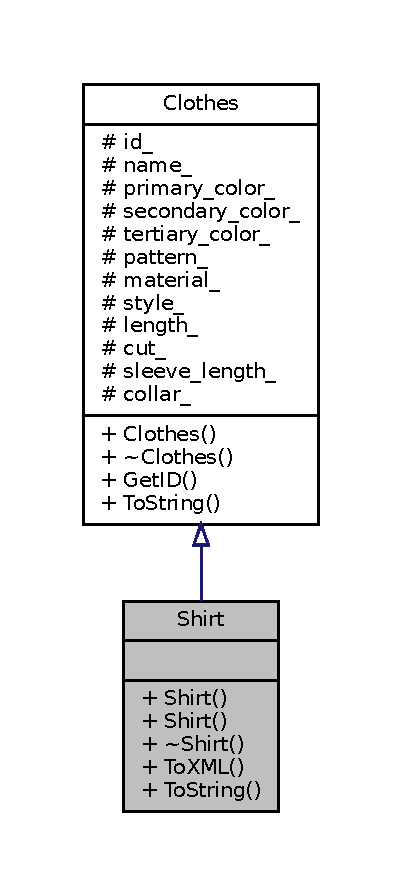
\includegraphics[width=193pt]{classShirt__inherit__graph}
\end{center}
\end{figure}


Collaboration diagram for Shirt\+:\nopagebreak
\begin{figure}[H]
\begin{center}
\leavevmode
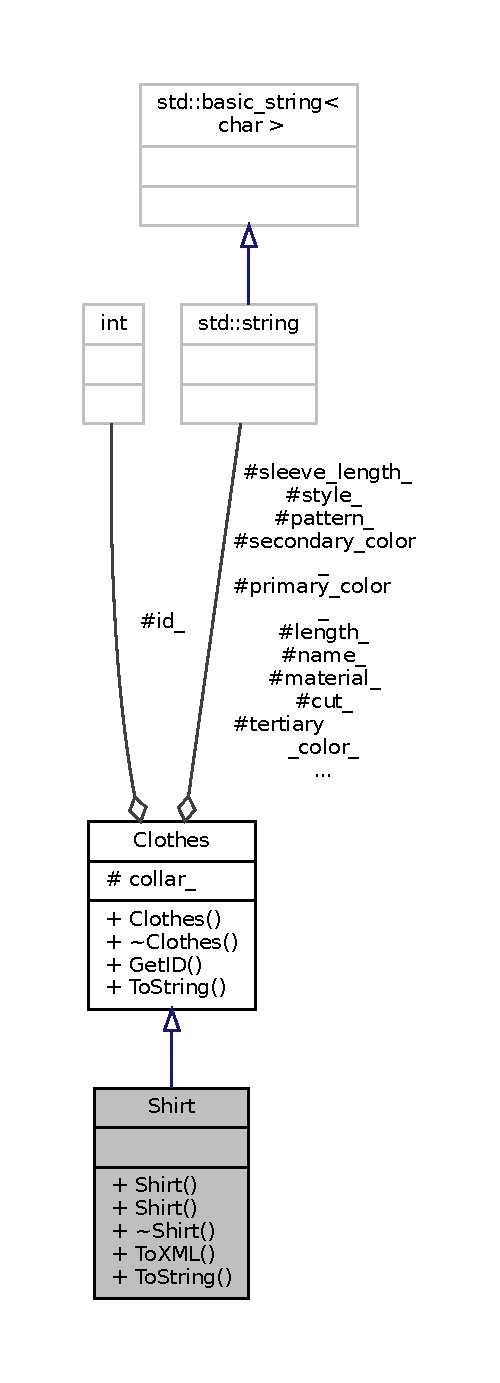
\includegraphics[height=550pt]{classShirt__coll__graph}
\end{center}
\end{figure}
\subsection*{Public Member Functions}
\begin{DoxyCompactItemize}
\item 
\mbox{\hyperlink{classShirt_a38664a136cdc92583d8c13a8281905d5}{Shirt}} ()
\item 
\mbox{\hyperlink{classShirt_a5df3975569b7f5874a905d31e4056b7b}{Shirt}} (int id, string name, string prim\+\_\+color, string sec\+\_\+color, string tert\+\_\+color, string pattern, string sleeve\+\_\+length, string collar)
\item 
virtual \mbox{\hyperlink{classShirt_a2cff1b945a014210e8bf009eb4269695}{$\sim$\+Shirt}} ()
\item 
string \mbox{\hyperlink{classShirt_ae636e58135bd1ca4ac590e55e8d47cac}{To\+X\+ML}} () const
\item 
string \mbox{\hyperlink{classShirt_ab85aaa20a603d63f4144d1b42d9b616d}{To\+String}} () const
\item 
int \mbox{\hyperlink{classClothes_a3f6dac172f333126d19010f85ec44e4c}{Get\+ID}} ()
\end{DoxyCompactItemize}
\subsection*{Protected Attributes}
\begin{DoxyCompactItemize}
\item 
int \mbox{\hyperlink{classClothes_a8978d931db5ca47c3ccea30def4ae83e}{id\+\_\+}} = \mbox{\hyperlink{clothes_8h_a77186917343a417a2369cdff0bc86d31}{k\+Dummy\+ID}}
\begin{DoxyCompactList}\small\item\em Global unique identifier. \end{DoxyCompactList}\item 
string \mbox{\hyperlink{classClothes_a7f2275aaae24224d60c48af922c31b65}{name\+\_\+}} = \mbox{\hyperlink{clothes_8h_adba739b5125fd5a4066ec0ef063c0657}{k\+Dummy\+Name}}
\begin{DoxyCompactList}\small\item\em User readable name. \end{DoxyCompactList}\item 
string \mbox{\hyperlink{classClothes_a7cb005bf6cbb7f4eaa40f1b31817559c}{primary\+\_\+color\+\_\+}} = \mbox{\hyperlink{clothes_8h_a1b9c685d3bf2811d95b65e0d396c1344}{k\+Dummy\+Prim\+Color}}
\begin{DoxyCompactList}\small\item\em Primary color. \end{DoxyCompactList}\item 
string \mbox{\hyperlink{classClothes_ab8f55f67b956b25d71260cffcf273673}{secondary\+\_\+color\+\_\+}} = \mbox{\hyperlink{clothes_8h_a71c39811135425d881af7760da63a73a}{k\+Dummy\+Sec\+Color}}
\begin{DoxyCompactList}\small\item\em Secondary color. \end{DoxyCompactList}\item 
string \mbox{\hyperlink{classClothes_a3c5f1e7ab531e3ba7a38b930da8078a0}{tertiary\+\_\+color\+\_\+}} = \mbox{\hyperlink{clothes_8h_a094dde85547895fd70dafb3ab10c6783}{k\+Dummy\+Tert\+Color}}
\begin{DoxyCompactList}\small\item\em Tertiary color. \end{DoxyCompactList}\item 
string \mbox{\hyperlink{classClothes_a1d40145a4eb6d28441f112f030ab5d35}{pattern\+\_\+}} = \mbox{\hyperlink{clothes_8h_a2e72ae4d77adb7bc9cbecf4dea1e9e22}{k\+Dummy\+Pattern}}
\begin{DoxyCompactList}\small\item\em Design pattern. \end{DoxyCompactList}\item 
string \mbox{\hyperlink{classClothes_adbb9ed311f14ccbb1e4fe0e8378a95d4}{material\+\_\+}} = \mbox{\hyperlink{clothes_8h_a9df1268c6668ae4e2a728ccf032cc33d}{k\+Dummy\+Material}}
\begin{DoxyCompactList}\small\item\em Material. \end{DoxyCompactList}\item 
string \mbox{\hyperlink{classClothes_aa85ed2b95110d8c477a1aca9cb403f98}{style\+\_\+}} = \mbox{\hyperlink{clothes_8h_a9deec6ed1f40928bfa0040eeab95ed6b}{k\+Dummy\+Style}}
\begin{DoxyCompactList}\small\item\em Design style. \end{DoxyCompactList}\item 
string \mbox{\hyperlink{classClothes_ae02603eda727e33caf46ec30e761e3c3}{length\+\_\+}} = \mbox{\hyperlink{clothes_8h_a1624256dcecfb0995a74c36142593770}{k\+Dummy\+Length}}
\begin{DoxyCompactList}\small\item\em Length of the clothing. \end{DoxyCompactList}\item 
string \mbox{\hyperlink{classClothes_ac1c2286c8928a5eee91d818a098a44ac}{cut\+\_\+}} = \mbox{\hyperlink{clothes_8h_a8a6eb066049b009439505355aeaae375}{k\+Dummy\+Cut}}
\begin{DoxyCompactList}\small\item\em Cut of the clothing. \end{DoxyCompactList}\item 
string \mbox{\hyperlink{classClothes_a012aeb71e62ebaf9b5b5dd700cc8d5db}{sleeve\+\_\+length\+\_\+}} = \mbox{\hyperlink{clothes_8h_a0f53dde6a2c4c344bb7da50655497350}{k\+Dummy\+Sleeve\+Length}}
\begin{DoxyCompactList}\small\item\em Length of the sleeve. \end{DoxyCompactList}\item 
string \mbox{\hyperlink{classClothes_ae2e5026257b3a2f2ddbf61757fd3b57b}{collar\+\_\+}} = \mbox{\hyperlink{clothes_8h_ac06c9f556f68bcd2829e36c55b70a86e}{k\+Dummy\+Collar}}
\begin{DoxyCompactList}\small\item\em Type of collar. \end{DoxyCompactList}\end{DoxyCompactItemize}


\subsection{Constructor \& Destructor Documentation}
\mbox{\Hypertarget{classShirt_a38664a136cdc92583d8c13a8281905d5}\label{classShirt_a38664a136cdc92583d8c13a8281905d5}} 
\index{Shirt@{Shirt}!Shirt@{Shirt}}
\index{Shirt@{Shirt}!Shirt@{Shirt}}
\subsubsection{\texorpdfstring{Shirt()}{Shirt()}\hspace{0.1cm}{\footnotesize\ttfamily [1/2]}}
{\footnotesize\ttfamily Shirt\+::\+Shirt (\begin{DoxyParamCaption}{ }\end{DoxyParamCaption})}

\mbox{\Hypertarget{classShirt_a5df3975569b7f5874a905d31e4056b7b}\label{classShirt_a5df3975569b7f5874a905d31e4056b7b}} 
\index{Shirt@{Shirt}!Shirt@{Shirt}}
\index{Shirt@{Shirt}!Shirt@{Shirt}}
\subsubsection{\texorpdfstring{Shirt()}{Shirt()}\hspace{0.1cm}{\footnotesize\ttfamily [2/2]}}
{\footnotesize\ttfamily Shirt\+::\+Shirt (\begin{DoxyParamCaption}\item[{int}]{id,  }\item[{string}]{name,  }\item[{string}]{prim\+\_\+color,  }\item[{string}]{sec\+\_\+color,  }\item[{string}]{tert\+\_\+color,  }\item[{string}]{pattern,  }\item[{string}]{sleeve\+\_\+length,  }\item[{string}]{collar }\end{DoxyParamCaption})}

\mbox{\Hypertarget{classShirt_a2cff1b945a014210e8bf009eb4269695}\label{classShirt_a2cff1b945a014210e8bf009eb4269695}} 
\index{Shirt@{Shirt}!````~Shirt@{$\sim$\+Shirt}}
\index{````~Shirt@{$\sim$\+Shirt}!Shirt@{Shirt}}
\subsubsection{\texorpdfstring{$\sim$\+Shirt()}{~Shirt()}}
{\footnotesize\ttfamily Shirt\+::$\sim$\+Shirt (\begin{DoxyParamCaption}{ }\end{DoxyParamCaption})\hspace{0.3cm}{\ttfamily [virtual]}}



\subsection{Member Function Documentation}
\mbox{\Hypertarget{classClothes_a3f6dac172f333126d19010f85ec44e4c}\label{classClothes_a3f6dac172f333126d19010f85ec44e4c}} 
\index{Shirt@{Shirt}!Get\+ID@{Get\+ID}}
\index{Get\+ID@{Get\+ID}!Shirt@{Shirt}}
\subsubsection{\texorpdfstring{Get\+I\+D()}{GetID()}}
{\footnotesize\ttfamily int Clothes\+::\+Get\+ID (\begin{DoxyParamCaption}{ }\end{DoxyParamCaption})\hspace{0.3cm}{\ttfamily [inline]}, {\ttfamily [inherited]}}

Here is the caller graph for this function\+:\nopagebreak
\begin{figure}[H]
\begin{center}
\leavevmode
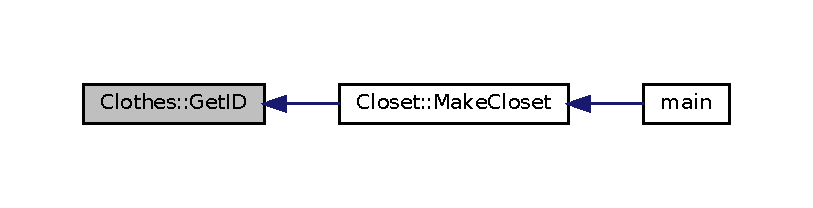
\includegraphics[width=350pt]{classClothes_a3f6dac172f333126d19010f85ec44e4c_icgraph}
\end{center}
\end{figure}
\mbox{\Hypertarget{classShirt_ab85aaa20a603d63f4144d1b42d9b616d}\label{classShirt_ab85aaa20a603d63f4144d1b42d9b616d}} 
\index{Shirt@{Shirt}!To\+String@{To\+String}}
\index{To\+String@{To\+String}!Shirt@{Shirt}}
\subsubsection{\texorpdfstring{To\+String()}{ToString()}}
{\footnotesize\ttfamily string Shirt\+::\+To\+String (\begin{DoxyParamCaption}{ }\end{DoxyParamCaption}) const\hspace{0.3cm}{\ttfamily [virtual]}}

This is what makes this a purely abstract class. The implementation of these will be changed from one article of clothing to the next. 

Implements \mbox{\hyperlink{classClothes_a953d143394e9a2c007ab0c3a638973cf}{Clothes}}.

\mbox{\Hypertarget{classShirt_ae636e58135bd1ca4ac590e55e8d47cac}\label{classShirt_ae636e58135bd1ca4ac590e55e8d47cac}} 
\index{Shirt@{Shirt}!To\+X\+ML@{To\+X\+ML}}
\index{To\+X\+ML@{To\+X\+ML}!Shirt@{Shirt}}
\subsubsection{\texorpdfstring{To\+X\+M\+L()}{ToXML()}}
{\footnotesize\ttfamily string Shirt\+::\+To\+X\+ML (\begin{DoxyParamCaption}{ }\end{DoxyParamCaption}) const}



\subsection{Member Data Documentation}
\mbox{\Hypertarget{classClothes_ae2e5026257b3a2f2ddbf61757fd3b57b}\label{classClothes_ae2e5026257b3a2f2ddbf61757fd3b57b}} 
\index{Shirt@{Shirt}!collar\+\_\+@{collar\+\_\+}}
\index{collar\+\_\+@{collar\+\_\+}!Shirt@{Shirt}}
\subsubsection{\texorpdfstring{collar\+\_\+}{collar\_}}
{\footnotesize\ttfamily string Clothes\+::collar\+\_\+ = \mbox{\hyperlink{clothes_8h_ac06c9f556f68bcd2829e36c55b70a86e}{k\+Dummy\+Collar}}\hspace{0.3cm}{\ttfamily [protected]}, {\ttfamily [inherited]}}



Type of collar. 

\mbox{\Hypertarget{classClothes_ac1c2286c8928a5eee91d818a098a44ac}\label{classClothes_ac1c2286c8928a5eee91d818a098a44ac}} 
\index{Shirt@{Shirt}!cut\+\_\+@{cut\+\_\+}}
\index{cut\+\_\+@{cut\+\_\+}!Shirt@{Shirt}}
\subsubsection{\texorpdfstring{cut\+\_\+}{cut\_}}
{\footnotesize\ttfamily string Clothes\+::cut\+\_\+ = \mbox{\hyperlink{clothes_8h_a8a6eb066049b009439505355aeaae375}{k\+Dummy\+Cut}}\hspace{0.3cm}{\ttfamily [protected]}, {\ttfamily [inherited]}}



Cut of the clothing. 

\mbox{\Hypertarget{classClothes_a8978d931db5ca47c3ccea30def4ae83e}\label{classClothes_a8978d931db5ca47c3ccea30def4ae83e}} 
\index{Shirt@{Shirt}!id\+\_\+@{id\+\_\+}}
\index{id\+\_\+@{id\+\_\+}!Shirt@{Shirt}}
\subsubsection{\texorpdfstring{id\+\_\+}{id\_}}
{\footnotesize\ttfamily int Clothes\+::id\+\_\+ = \mbox{\hyperlink{clothes_8h_a77186917343a417a2369cdff0bc86d31}{k\+Dummy\+ID}}\hspace{0.3cm}{\ttfamily [protected]}, {\ttfamily [inherited]}}



Global unique identifier. 

\mbox{\Hypertarget{classClothes_ae02603eda727e33caf46ec30e761e3c3}\label{classClothes_ae02603eda727e33caf46ec30e761e3c3}} 
\index{Shirt@{Shirt}!length\+\_\+@{length\+\_\+}}
\index{length\+\_\+@{length\+\_\+}!Shirt@{Shirt}}
\subsubsection{\texorpdfstring{length\+\_\+}{length\_}}
{\footnotesize\ttfamily string Clothes\+::length\+\_\+ = \mbox{\hyperlink{clothes_8h_a1624256dcecfb0995a74c36142593770}{k\+Dummy\+Length}}\hspace{0.3cm}{\ttfamily [protected]}, {\ttfamily [inherited]}}



Length of the clothing. 

\mbox{\Hypertarget{classClothes_adbb9ed311f14ccbb1e4fe0e8378a95d4}\label{classClothes_adbb9ed311f14ccbb1e4fe0e8378a95d4}} 
\index{Shirt@{Shirt}!material\+\_\+@{material\+\_\+}}
\index{material\+\_\+@{material\+\_\+}!Shirt@{Shirt}}
\subsubsection{\texorpdfstring{material\+\_\+}{material\_}}
{\footnotesize\ttfamily string Clothes\+::material\+\_\+ = \mbox{\hyperlink{clothes_8h_a9df1268c6668ae4e2a728ccf032cc33d}{k\+Dummy\+Material}}\hspace{0.3cm}{\ttfamily [protected]}, {\ttfamily [inherited]}}



Material. 

\mbox{\Hypertarget{classClothes_a7f2275aaae24224d60c48af922c31b65}\label{classClothes_a7f2275aaae24224d60c48af922c31b65}} 
\index{Shirt@{Shirt}!name\+\_\+@{name\+\_\+}}
\index{name\+\_\+@{name\+\_\+}!Shirt@{Shirt}}
\subsubsection{\texorpdfstring{name\+\_\+}{name\_}}
{\footnotesize\ttfamily string Clothes\+::name\+\_\+ = \mbox{\hyperlink{clothes_8h_adba739b5125fd5a4066ec0ef063c0657}{k\+Dummy\+Name}}\hspace{0.3cm}{\ttfamily [protected]}, {\ttfamily [inherited]}}



User readable name. 

\mbox{\Hypertarget{classClothes_a1d40145a4eb6d28441f112f030ab5d35}\label{classClothes_a1d40145a4eb6d28441f112f030ab5d35}} 
\index{Shirt@{Shirt}!pattern\+\_\+@{pattern\+\_\+}}
\index{pattern\+\_\+@{pattern\+\_\+}!Shirt@{Shirt}}
\subsubsection{\texorpdfstring{pattern\+\_\+}{pattern\_}}
{\footnotesize\ttfamily string Clothes\+::pattern\+\_\+ = \mbox{\hyperlink{clothes_8h_a2e72ae4d77adb7bc9cbecf4dea1e9e22}{k\+Dummy\+Pattern}}\hspace{0.3cm}{\ttfamily [protected]}, {\ttfamily [inherited]}}



Design pattern. 

\mbox{\Hypertarget{classClothes_a7cb005bf6cbb7f4eaa40f1b31817559c}\label{classClothes_a7cb005bf6cbb7f4eaa40f1b31817559c}} 
\index{Shirt@{Shirt}!primary\+\_\+color\+\_\+@{primary\+\_\+color\+\_\+}}
\index{primary\+\_\+color\+\_\+@{primary\+\_\+color\+\_\+}!Shirt@{Shirt}}
\subsubsection{\texorpdfstring{primary\+\_\+color\+\_\+}{primary\_color\_}}
{\footnotesize\ttfamily string Clothes\+::primary\+\_\+color\+\_\+ = \mbox{\hyperlink{clothes_8h_a1b9c685d3bf2811d95b65e0d396c1344}{k\+Dummy\+Prim\+Color}}\hspace{0.3cm}{\ttfamily [protected]}, {\ttfamily [inherited]}}



Primary color. 

\mbox{\Hypertarget{classClothes_ab8f55f67b956b25d71260cffcf273673}\label{classClothes_ab8f55f67b956b25d71260cffcf273673}} 
\index{Shirt@{Shirt}!secondary\+\_\+color\+\_\+@{secondary\+\_\+color\+\_\+}}
\index{secondary\+\_\+color\+\_\+@{secondary\+\_\+color\+\_\+}!Shirt@{Shirt}}
\subsubsection{\texorpdfstring{secondary\+\_\+color\+\_\+}{secondary\_color\_}}
{\footnotesize\ttfamily string Clothes\+::secondary\+\_\+color\+\_\+ = \mbox{\hyperlink{clothes_8h_a71c39811135425d881af7760da63a73a}{k\+Dummy\+Sec\+Color}}\hspace{0.3cm}{\ttfamily [protected]}, {\ttfamily [inherited]}}



Secondary color. 

\mbox{\Hypertarget{classClothes_a012aeb71e62ebaf9b5b5dd700cc8d5db}\label{classClothes_a012aeb71e62ebaf9b5b5dd700cc8d5db}} 
\index{Shirt@{Shirt}!sleeve\+\_\+length\+\_\+@{sleeve\+\_\+length\+\_\+}}
\index{sleeve\+\_\+length\+\_\+@{sleeve\+\_\+length\+\_\+}!Shirt@{Shirt}}
\subsubsection{\texorpdfstring{sleeve\+\_\+length\+\_\+}{sleeve\_length\_}}
{\footnotesize\ttfamily string Clothes\+::sleeve\+\_\+length\+\_\+ = \mbox{\hyperlink{clothes_8h_a0f53dde6a2c4c344bb7da50655497350}{k\+Dummy\+Sleeve\+Length}}\hspace{0.3cm}{\ttfamily [protected]}, {\ttfamily [inherited]}}



Length of the sleeve. 

\mbox{\Hypertarget{classClothes_aa85ed2b95110d8c477a1aca9cb403f98}\label{classClothes_aa85ed2b95110d8c477a1aca9cb403f98}} 
\index{Shirt@{Shirt}!style\+\_\+@{style\+\_\+}}
\index{style\+\_\+@{style\+\_\+}!Shirt@{Shirt}}
\subsubsection{\texorpdfstring{style\+\_\+}{style\_}}
{\footnotesize\ttfamily string Clothes\+::style\+\_\+ = \mbox{\hyperlink{clothes_8h_a9deec6ed1f40928bfa0040eeab95ed6b}{k\+Dummy\+Style}}\hspace{0.3cm}{\ttfamily [protected]}, {\ttfamily [inherited]}}



Design style. 

\mbox{\Hypertarget{classClothes_a3c5f1e7ab531e3ba7a38b930da8078a0}\label{classClothes_a3c5f1e7ab531e3ba7a38b930da8078a0}} 
\index{Shirt@{Shirt}!tertiary\+\_\+color\+\_\+@{tertiary\+\_\+color\+\_\+}}
\index{tertiary\+\_\+color\+\_\+@{tertiary\+\_\+color\+\_\+}!Shirt@{Shirt}}
\subsubsection{\texorpdfstring{tertiary\+\_\+color\+\_\+}{tertiary\_color\_}}
{\footnotesize\ttfamily string Clothes\+::tertiary\+\_\+color\+\_\+ = \mbox{\hyperlink{clothes_8h_a094dde85547895fd70dafb3ab10c6783}{k\+Dummy\+Tert\+Color}}\hspace{0.3cm}{\ttfamily [protected]}, {\ttfamily [inherited]}}



Tertiary color. 



The documentation for this class was generated from the following files\+:\begin{DoxyCompactItemize}
\item 
\mbox{\hyperlink{shirt_8h}{shirt.\+h}}\item 
\mbox{\hyperlink{shirt_8cc}{shirt.\+cc}}\end{DoxyCompactItemize}

\hypertarget{classShoes}{}\section{Shoes Class Reference}
\label{classShoes}\index{Shoes@{Shoes}}


{\ttfamily \#include $<$shoes.\+h$>$}



Inheritance diagram for Shoes\+:\nopagebreak
\begin{figure}[H]
\begin{center}
\leavevmode
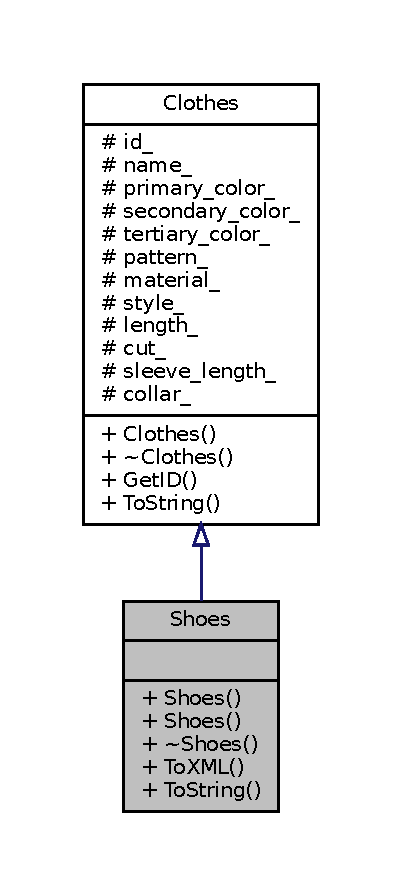
\includegraphics[width=193pt]{classShoes__inherit__graph}
\end{center}
\end{figure}


Collaboration diagram for Shoes\+:\nopagebreak
\begin{figure}[H]
\begin{center}
\leavevmode
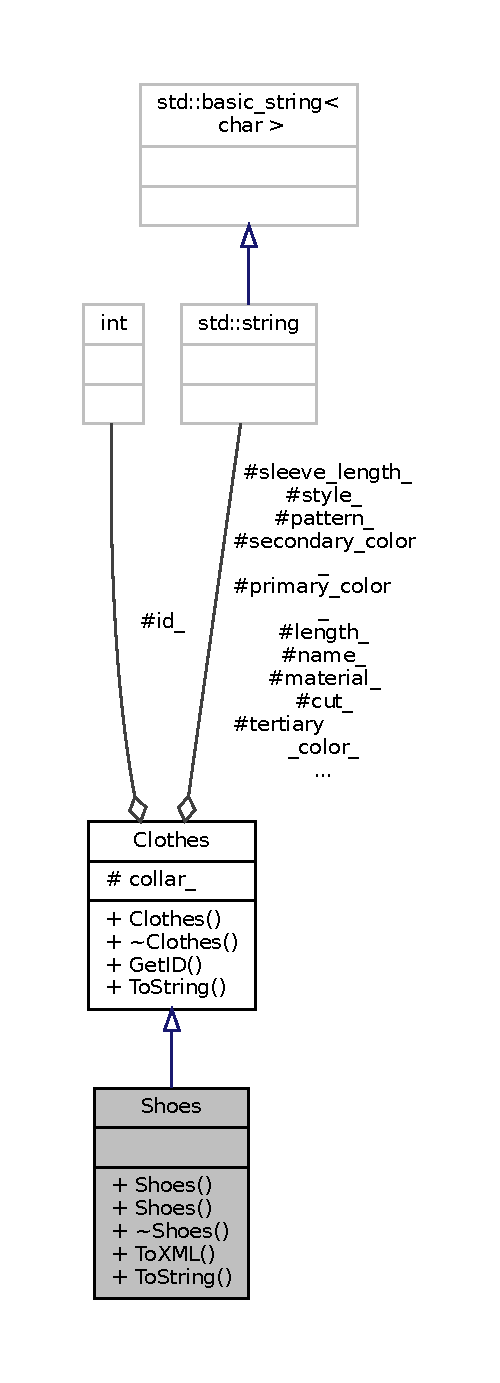
\includegraphics[height=550pt]{classShoes__coll__graph}
\end{center}
\end{figure}
\subsection*{Public Member Functions}
\begin{DoxyCompactItemize}
\item 
\mbox{\hyperlink{classShoes_af27b3cc545cf835d7a2eb5817347506a}{Shoes}} ()
\item 
\mbox{\hyperlink{classShoes_a4f38fcd11c63cf3256c9688cf1bd19b3}{Shoes}} (int id, string name, string prim\+\_\+color, string sec\+\_\+color, string tert\+\_\+color, string material, string style)
\item 
virtual \mbox{\hyperlink{classShoes_afc511aaebac8e7ab57286cf35db7ce8f}{$\sim$\+Shoes}} ()
\item 
string \mbox{\hyperlink{classShoes_acf6f049aa995a189b0f892f86defeefd}{To\+X\+ML}} () const
\item 
string \mbox{\hyperlink{classShoes_a9b1bcc00ec7ef920d34bf9193c96a1ce}{To\+String}} () const
\item 
int \mbox{\hyperlink{classClothes_a3f6dac172f333126d19010f85ec44e4c}{Get\+ID}} ()
\end{DoxyCompactItemize}
\subsection*{Protected Attributes}
\begin{DoxyCompactItemize}
\item 
int \mbox{\hyperlink{classClothes_a8978d931db5ca47c3ccea30def4ae83e}{id\+\_\+}} = \mbox{\hyperlink{clothes_8h_a77186917343a417a2369cdff0bc86d31}{k\+Dummy\+ID}}
\begin{DoxyCompactList}\small\item\em Global unique identifier. \end{DoxyCompactList}\item 
string \mbox{\hyperlink{classClothes_a7f2275aaae24224d60c48af922c31b65}{name\+\_\+}} = \mbox{\hyperlink{clothes_8h_adba739b5125fd5a4066ec0ef063c0657}{k\+Dummy\+Name}}
\begin{DoxyCompactList}\small\item\em User readable name. \end{DoxyCompactList}\item 
string \mbox{\hyperlink{classClothes_a7cb005bf6cbb7f4eaa40f1b31817559c}{primary\+\_\+color\+\_\+}} = \mbox{\hyperlink{clothes_8h_a1b9c685d3bf2811d95b65e0d396c1344}{k\+Dummy\+Prim\+Color}}
\begin{DoxyCompactList}\small\item\em Primary color. \end{DoxyCompactList}\item 
string \mbox{\hyperlink{classClothes_ab8f55f67b956b25d71260cffcf273673}{secondary\+\_\+color\+\_\+}} = \mbox{\hyperlink{clothes_8h_a71c39811135425d881af7760da63a73a}{k\+Dummy\+Sec\+Color}}
\begin{DoxyCompactList}\small\item\em Secondary color. \end{DoxyCompactList}\item 
string \mbox{\hyperlink{classClothes_a3c5f1e7ab531e3ba7a38b930da8078a0}{tertiary\+\_\+color\+\_\+}} = \mbox{\hyperlink{clothes_8h_a094dde85547895fd70dafb3ab10c6783}{k\+Dummy\+Tert\+Color}}
\begin{DoxyCompactList}\small\item\em Tertiary color. \end{DoxyCompactList}\item 
string \mbox{\hyperlink{classClothes_a1d40145a4eb6d28441f112f030ab5d35}{pattern\+\_\+}} = \mbox{\hyperlink{clothes_8h_a2e72ae4d77adb7bc9cbecf4dea1e9e22}{k\+Dummy\+Pattern}}
\begin{DoxyCompactList}\small\item\em Design pattern. \end{DoxyCompactList}\item 
string \mbox{\hyperlink{classClothes_adbb9ed311f14ccbb1e4fe0e8378a95d4}{material\+\_\+}} = \mbox{\hyperlink{clothes_8h_a9df1268c6668ae4e2a728ccf032cc33d}{k\+Dummy\+Material}}
\begin{DoxyCompactList}\small\item\em Material. \end{DoxyCompactList}\item 
string \mbox{\hyperlink{classClothes_aa85ed2b95110d8c477a1aca9cb403f98}{style\+\_\+}} = \mbox{\hyperlink{clothes_8h_a9deec6ed1f40928bfa0040eeab95ed6b}{k\+Dummy\+Style}}
\begin{DoxyCompactList}\small\item\em Design style. \end{DoxyCompactList}\item 
string \mbox{\hyperlink{classClothes_ae02603eda727e33caf46ec30e761e3c3}{length\+\_\+}} = \mbox{\hyperlink{clothes_8h_a1624256dcecfb0995a74c36142593770}{k\+Dummy\+Length}}
\begin{DoxyCompactList}\small\item\em Length of the clothing. \end{DoxyCompactList}\item 
string \mbox{\hyperlink{classClothes_ac1c2286c8928a5eee91d818a098a44ac}{cut\+\_\+}} = \mbox{\hyperlink{clothes_8h_a8a6eb066049b009439505355aeaae375}{k\+Dummy\+Cut}}
\begin{DoxyCompactList}\small\item\em Cut of the clothing. \end{DoxyCompactList}\item 
string \mbox{\hyperlink{classClothes_a012aeb71e62ebaf9b5b5dd700cc8d5db}{sleeve\+\_\+length\+\_\+}} = \mbox{\hyperlink{clothes_8h_a0f53dde6a2c4c344bb7da50655497350}{k\+Dummy\+Sleeve\+Length}}
\begin{DoxyCompactList}\small\item\em Length of the sleeve. \end{DoxyCompactList}\item 
string \mbox{\hyperlink{classClothes_ae2e5026257b3a2f2ddbf61757fd3b57b}{collar\+\_\+}} = \mbox{\hyperlink{clothes_8h_ac06c9f556f68bcd2829e36c55b70a86e}{k\+Dummy\+Collar}}
\begin{DoxyCompactList}\small\item\em Type of collar. \end{DoxyCompactList}\end{DoxyCompactItemize}


\subsection{Constructor \& Destructor Documentation}
\mbox{\Hypertarget{classShoes_af27b3cc545cf835d7a2eb5817347506a}\label{classShoes_af27b3cc545cf835d7a2eb5817347506a}} 
\index{Shoes@{Shoes}!Shoes@{Shoes}}
\index{Shoes@{Shoes}!Shoes@{Shoes}}
\subsubsection{\texorpdfstring{Shoes()}{Shoes()}\hspace{0.1cm}{\footnotesize\ttfamily [1/2]}}
{\footnotesize\ttfamily Shoes\+::\+Shoes (\begin{DoxyParamCaption}{ }\end{DoxyParamCaption})}

\mbox{\Hypertarget{classShoes_a4f38fcd11c63cf3256c9688cf1bd19b3}\label{classShoes_a4f38fcd11c63cf3256c9688cf1bd19b3}} 
\index{Shoes@{Shoes}!Shoes@{Shoes}}
\index{Shoes@{Shoes}!Shoes@{Shoes}}
\subsubsection{\texorpdfstring{Shoes()}{Shoes()}\hspace{0.1cm}{\footnotesize\ttfamily [2/2]}}
{\footnotesize\ttfamily Shoes\+::\+Shoes (\begin{DoxyParamCaption}\item[{int}]{id,  }\item[{string}]{name,  }\item[{string}]{prim\+\_\+color,  }\item[{string}]{sec\+\_\+color,  }\item[{string}]{tert\+\_\+color,  }\item[{string}]{material,  }\item[{string}]{style }\end{DoxyParamCaption})}



References \mbox{\hyperlink{classClothes_a8978d931db5ca47c3ccea30def4ae83e}{Clothes\+::id\+\_\+}}, \mbox{\hyperlink{classClothes_adbb9ed311f14ccbb1e4fe0e8378a95d4}{Clothes\+::material\+\_\+}}, \mbox{\hyperlink{classClothes_a7f2275aaae24224d60c48af922c31b65}{Clothes\+::name\+\_\+}}, \mbox{\hyperlink{classClothes_a7cb005bf6cbb7f4eaa40f1b31817559c}{Clothes\+::primary\+\_\+color\+\_\+}}, \mbox{\hyperlink{classClothes_ab8f55f67b956b25d71260cffcf273673}{Clothes\+::secondary\+\_\+color\+\_\+}}, \mbox{\hyperlink{classClothes_aa85ed2b95110d8c477a1aca9cb403f98}{Clothes\+::style\+\_\+}}, and \mbox{\hyperlink{classClothes_a3c5f1e7ab531e3ba7a38b930da8078a0}{Clothes\+::tertiary\+\_\+color\+\_\+}}.

\mbox{\Hypertarget{classShoes_afc511aaebac8e7ab57286cf35db7ce8f}\label{classShoes_afc511aaebac8e7ab57286cf35db7ce8f}} 
\index{Shoes@{Shoes}!````~Shoes@{$\sim$\+Shoes}}
\index{````~Shoes@{$\sim$\+Shoes}!Shoes@{Shoes}}
\subsubsection{\texorpdfstring{$\sim$\+Shoes()}{~Shoes()}}
{\footnotesize\ttfamily Shoes\+::$\sim$\+Shoes (\begin{DoxyParamCaption}{ }\end{DoxyParamCaption})\hspace{0.3cm}{\ttfamily [virtual]}}



\subsection{Member Function Documentation}
\mbox{\Hypertarget{classClothes_a3f6dac172f333126d19010f85ec44e4c}\label{classClothes_a3f6dac172f333126d19010f85ec44e4c}} 
\index{Shoes@{Shoes}!Get\+ID@{Get\+ID}}
\index{Get\+ID@{Get\+ID}!Shoes@{Shoes}}
\subsubsection{\texorpdfstring{Get\+I\+D()}{GetID()}}
{\footnotesize\ttfamily int Clothes\+::\+Get\+ID (\begin{DoxyParamCaption}{ }\end{DoxyParamCaption})\hspace{0.3cm}{\ttfamily [inline]}, {\ttfamily [inherited]}}

Here is the caller graph for this function\+:\nopagebreak
\begin{figure}[H]
\begin{center}
\leavevmode
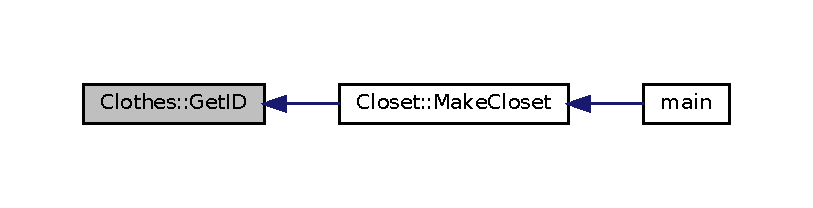
\includegraphics[width=350pt]{classClothes_a3f6dac172f333126d19010f85ec44e4c_icgraph}
\end{center}
\end{figure}
\mbox{\Hypertarget{classShoes_a9b1bcc00ec7ef920d34bf9193c96a1ce}\label{classShoes_a9b1bcc00ec7ef920d34bf9193c96a1ce}} 
\index{Shoes@{Shoes}!To\+String@{To\+String}}
\index{To\+String@{To\+String}!Shoes@{Shoes}}
\subsubsection{\texorpdfstring{To\+String()}{ToString()}}
{\footnotesize\ttfamily string Shoes\+::\+To\+String (\begin{DoxyParamCaption}{ }\end{DoxyParamCaption}) const\hspace{0.3cm}{\ttfamily [virtual]}}

This is what makes this a purely abstract class. The implementation of these will be changed from one article of clothing to the next. 

Implements \mbox{\hyperlink{classClothes_a953d143394e9a2c007ab0c3a638973cf}{Clothes}}.



References \mbox{\hyperlink{classClothes_a8978d931db5ca47c3ccea30def4ae83e}{Clothes\+::id\+\_\+}}, \mbox{\hyperlink{classClothes_adbb9ed311f14ccbb1e4fe0e8378a95d4}{Clothes\+::material\+\_\+}}, \mbox{\hyperlink{classClothes_a7f2275aaae24224d60c48af922c31b65}{Clothes\+::name\+\_\+}}, \mbox{\hyperlink{classClothes_a7cb005bf6cbb7f4eaa40f1b31817559c}{Clothes\+::primary\+\_\+color\+\_\+}}, \mbox{\hyperlink{classClothes_ab8f55f67b956b25d71260cffcf273673}{Clothes\+::secondary\+\_\+color\+\_\+}}, \mbox{\hyperlink{classClothes_aa85ed2b95110d8c477a1aca9cb403f98}{Clothes\+::style\+\_\+}}, and \mbox{\hyperlink{classClothes_a3c5f1e7ab531e3ba7a38b930da8078a0}{Clothes\+::tertiary\+\_\+color\+\_\+}}.

\mbox{\Hypertarget{classShoes_acf6f049aa995a189b0f892f86defeefd}\label{classShoes_acf6f049aa995a189b0f892f86defeefd}} 
\index{Shoes@{Shoes}!To\+X\+ML@{To\+X\+ML}}
\index{To\+X\+ML@{To\+X\+ML}!Shoes@{Shoes}}
\subsubsection{\texorpdfstring{To\+X\+M\+L()}{ToXML()}}
{\footnotesize\ttfamily string Shoes\+::\+To\+X\+ML (\begin{DoxyParamCaption}{ }\end{DoxyParamCaption}) const}



References \mbox{\hyperlink{classClothes_a8978d931db5ca47c3ccea30def4ae83e}{Clothes\+::id\+\_\+}}, \mbox{\hyperlink{classClothes_adbb9ed311f14ccbb1e4fe0e8378a95d4}{Clothes\+::material\+\_\+}}, \mbox{\hyperlink{classClothes_a7f2275aaae24224d60c48af922c31b65}{Clothes\+::name\+\_\+}}, \mbox{\hyperlink{classClothes_a7cb005bf6cbb7f4eaa40f1b31817559c}{Clothes\+::primary\+\_\+color\+\_\+}}, \mbox{\hyperlink{classClothes_ab8f55f67b956b25d71260cffcf273673}{Clothes\+::secondary\+\_\+color\+\_\+}}, \mbox{\hyperlink{classClothes_aa85ed2b95110d8c477a1aca9cb403f98}{Clothes\+::style\+\_\+}}, and \mbox{\hyperlink{classClothes_a3c5f1e7ab531e3ba7a38b930da8078a0}{Clothes\+::tertiary\+\_\+color\+\_\+}}.



\subsection{Member Data Documentation}
\mbox{\Hypertarget{classClothes_ae2e5026257b3a2f2ddbf61757fd3b57b}\label{classClothes_ae2e5026257b3a2f2ddbf61757fd3b57b}} 
\index{Shoes@{Shoes}!collar\+\_\+@{collar\+\_\+}}
\index{collar\+\_\+@{collar\+\_\+}!Shoes@{Shoes}}
\subsubsection{\texorpdfstring{collar\+\_\+}{collar\_}}
{\footnotesize\ttfamily string Clothes\+::collar\+\_\+ = \mbox{\hyperlink{clothes_8h_ac06c9f556f68bcd2829e36c55b70a86e}{k\+Dummy\+Collar}}\hspace{0.3cm}{\ttfamily [protected]}, {\ttfamily [inherited]}}



Type of collar. 

\mbox{\Hypertarget{classClothes_ac1c2286c8928a5eee91d818a098a44ac}\label{classClothes_ac1c2286c8928a5eee91d818a098a44ac}} 
\index{Shoes@{Shoes}!cut\+\_\+@{cut\+\_\+}}
\index{cut\+\_\+@{cut\+\_\+}!Shoes@{Shoes}}
\subsubsection{\texorpdfstring{cut\+\_\+}{cut\_}}
{\footnotesize\ttfamily string Clothes\+::cut\+\_\+ = \mbox{\hyperlink{clothes_8h_a8a6eb066049b009439505355aeaae375}{k\+Dummy\+Cut}}\hspace{0.3cm}{\ttfamily [protected]}, {\ttfamily [inherited]}}



Cut of the clothing. 

\mbox{\Hypertarget{classClothes_a8978d931db5ca47c3ccea30def4ae83e}\label{classClothes_a8978d931db5ca47c3ccea30def4ae83e}} 
\index{Shoes@{Shoes}!id\+\_\+@{id\+\_\+}}
\index{id\+\_\+@{id\+\_\+}!Shoes@{Shoes}}
\subsubsection{\texorpdfstring{id\+\_\+}{id\_}}
{\footnotesize\ttfamily int Clothes\+::id\+\_\+ = \mbox{\hyperlink{clothes_8h_a77186917343a417a2369cdff0bc86d31}{k\+Dummy\+ID}}\hspace{0.3cm}{\ttfamily [protected]}, {\ttfamily [inherited]}}



Global unique identifier. 

\mbox{\Hypertarget{classClothes_ae02603eda727e33caf46ec30e761e3c3}\label{classClothes_ae02603eda727e33caf46ec30e761e3c3}} 
\index{Shoes@{Shoes}!length\+\_\+@{length\+\_\+}}
\index{length\+\_\+@{length\+\_\+}!Shoes@{Shoes}}
\subsubsection{\texorpdfstring{length\+\_\+}{length\_}}
{\footnotesize\ttfamily string Clothes\+::length\+\_\+ = \mbox{\hyperlink{clothes_8h_a1624256dcecfb0995a74c36142593770}{k\+Dummy\+Length}}\hspace{0.3cm}{\ttfamily [protected]}, {\ttfamily [inherited]}}



Length of the clothing. 

\mbox{\Hypertarget{classClothes_adbb9ed311f14ccbb1e4fe0e8378a95d4}\label{classClothes_adbb9ed311f14ccbb1e4fe0e8378a95d4}} 
\index{Shoes@{Shoes}!material\+\_\+@{material\+\_\+}}
\index{material\+\_\+@{material\+\_\+}!Shoes@{Shoes}}
\subsubsection{\texorpdfstring{material\+\_\+}{material\_}}
{\footnotesize\ttfamily string Clothes\+::material\+\_\+ = \mbox{\hyperlink{clothes_8h_a9df1268c6668ae4e2a728ccf032cc33d}{k\+Dummy\+Material}}\hspace{0.3cm}{\ttfamily [protected]}, {\ttfamily [inherited]}}



Material. 

\mbox{\Hypertarget{classClothes_a7f2275aaae24224d60c48af922c31b65}\label{classClothes_a7f2275aaae24224d60c48af922c31b65}} 
\index{Shoes@{Shoes}!name\+\_\+@{name\+\_\+}}
\index{name\+\_\+@{name\+\_\+}!Shoes@{Shoes}}
\subsubsection{\texorpdfstring{name\+\_\+}{name\_}}
{\footnotesize\ttfamily string Clothes\+::name\+\_\+ = \mbox{\hyperlink{clothes_8h_adba739b5125fd5a4066ec0ef063c0657}{k\+Dummy\+Name}}\hspace{0.3cm}{\ttfamily [protected]}, {\ttfamily [inherited]}}



User readable name. 

\mbox{\Hypertarget{classClothes_a1d40145a4eb6d28441f112f030ab5d35}\label{classClothes_a1d40145a4eb6d28441f112f030ab5d35}} 
\index{Shoes@{Shoes}!pattern\+\_\+@{pattern\+\_\+}}
\index{pattern\+\_\+@{pattern\+\_\+}!Shoes@{Shoes}}
\subsubsection{\texorpdfstring{pattern\+\_\+}{pattern\_}}
{\footnotesize\ttfamily string Clothes\+::pattern\+\_\+ = \mbox{\hyperlink{clothes_8h_a2e72ae4d77adb7bc9cbecf4dea1e9e22}{k\+Dummy\+Pattern}}\hspace{0.3cm}{\ttfamily [protected]}, {\ttfamily [inherited]}}



Design pattern. 

\mbox{\Hypertarget{classClothes_a7cb005bf6cbb7f4eaa40f1b31817559c}\label{classClothes_a7cb005bf6cbb7f4eaa40f1b31817559c}} 
\index{Shoes@{Shoes}!primary\+\_\+color\+\_\+@{primary\+\_\+color\+\_\+}}
\index{primary\+\_\+color\+\_\+@{primary\+\_\+color\+\_\+}!Shoes@{Shoes}}
\subsubsection{\texorpdfstring{primary\+\_\+color\+\_\+}{primary\_color\_}}
{\footnotesize\ttfamily string Clothes\+::primary\+\_\+color\+\_\+ = \mbox{\hyperlink{clothes_8h_a1b9c685d3bf2811d95b65e0d396c1344}{k\+Dummy\+Prim\+Color}}\hspace{0.3cm}{\ttfamily [protected]}, {\ttfamily [inherited]}}



Primary color. 

\mbox{\Hypertarget{classClothes_ab8f55f67b956b25d71260cffcf273673}\label{classClothes_ab8f55f67b956b25d71260cffcf273673}} 
\index{Shoes@{Shoes}!secondary\+\_\+color\+\_\+@{secondary\+\_\+color\+\_\+}}
\index{secondary\+\_\+color\+\_\+@{secondary\+\_\+color\+\_\+}!Shoes@{Shoes}}
\subsubsection{\texorpdfstring{secondary\+\_\+color\+\_\+}{secondary\_color\_}}
{\footnotesize\ttfamily string Clothes\+::secondary\+\_\+color\+\_\+ = \mbox{\hyperlink{clothes_8h_a71c39811135425d881af7760da63a73a}{k\+Dummy\+Sec\+Color}}\hspace{0.3cm}{\ttfamily [protected]}, {\ttfamily [inherited]}}



Secondary color. 

\mbox{\Hypertarget{classClothes_a012aeb71e62ebaf9b5b5dd700cc8d5db}\label{classClothes_a012aeb71e62ebaf9b5b5dd700cc8d5db}} 
\index{Shoes@{Shoes}!sleeve\+\_\+length\+\_\+@{sleeve\+\_\+length\+\_\+}}
\index{sleeve\+\_\+length\+\_\+@{sleeve\+\_\+length\+\_\+}!Shoes@{Shoes}}
\subsubsection{\texorpdfstring{sleeve\+\_\+length\+\_\+}{sleeve\_length\_}}
{\footnotesize\ttfamily string Clothes\+::sleeve\+\_\+length\+\_\+ = \mbox{\hyperlink{clothes_8h_a0f53dde6a2c4c344bb7da50655497350}{k\+Dummy\+Sleeve\+Length}}\hspace{0.3cm}{\ttfamily [protected]}, {\ttfamily [inherited]}}



Length of the sleeve. 

\mbox{\Hypertarget{classClothes_aa85ed2b95110d8c477a1aca9cb403f98}\label{classClothes_aa85ed2b95110d8c477a1aca9cb403f98}} 
\index{Shoes@{Shoes}!style\+\_\+@{style\+\_\+}}
\index{style\+\_\+@{style\+\_\+}!Shoes@{Shoes}}
\subsubsection{\texorpdfstring{style\+\_\+}{style\_}}
{\footnotesize\ttfamily string Clothes\+::style\+\_\+ = \mbox{\hyperlink{clothes_8h_a9deec6ed1f40928bfa0040eeab95ed6b}{k\+Dummy\+Style}}\hspace{0.3cm}{\ttfamily [protected]}, {\ttfamily [inherited]}}



Design style. 

\mbox{\Hypertarget{classClothes_a3c5f1e7ab531e3ba7a38b930da8078a0}\label{classClothes_a3c5f1e7ab531e3ba7a38b930da8078a0}} 
\index{Shoes@{Shoes}!tertiary\+\_\+color\+\_\+@{tertiary\+\_\+color\+\_\+}}
\index{tertiary\+\_\+color\+\_\+@{tertiary\+\_\+color\+\_\+}!Shoes@{Shoes}}
\subsubsection{\texorpdfstring{tertiary\+\_\+color\+\_\+}{tertiary\_color\_}}
{\footnotesize\ttfamily string Clothes\+::tertiary\+\_\+color\+\_\+ = \mbox{\hyperlink{clothes_8h_a094dde85547895fd70dafb3ab10c6783}{k\+Dummy\+Tert\+Color}}\hspace{0.3cm}{\ttfamily [protected]}, {\ttfamily [inherited]}}



Tertiary color. 



The documentation for this class was generated from the following files\+:\begin{DoxyCompactItemize}
\item 
\mbox{\hyperlink{shoes_8h}{shoes.\+h}}\item 
\mbox{\hyperlink{shoes_8cc}{shoes.\+cc}}\end{DoxyCompactItemize}

\hypertarget{classSocks}{}\section{Socks Class Reference}
\label{classSocks}\index{Socks@{Socks}}


{\ttfamily \#include $<$socks.\+h$>$}



Inheritance diagram for Socks\+:\nopagebreak
\begin{figure}[H]
\begin{center}
\leavevmode
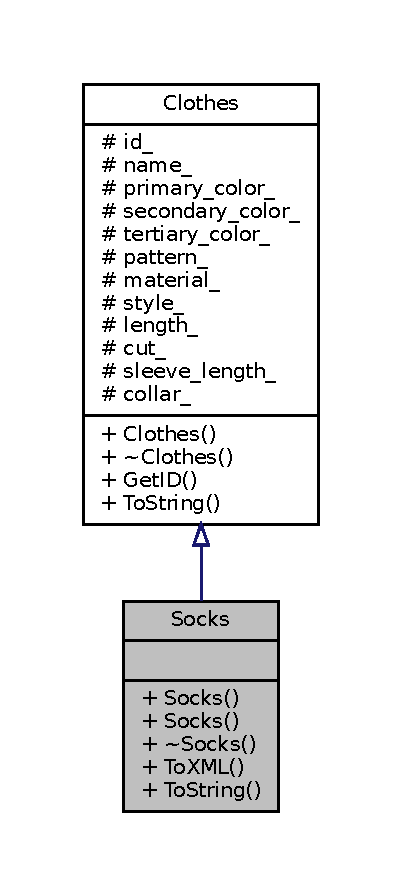
\includegraphics[width=193pt]{classSocks__inherit__graph}
\end{center}
\end{figure}


Collaboration diagram for Socks\+:\nopagebreak
\begin{figure}[H]
\begin{center}
\leavevmode
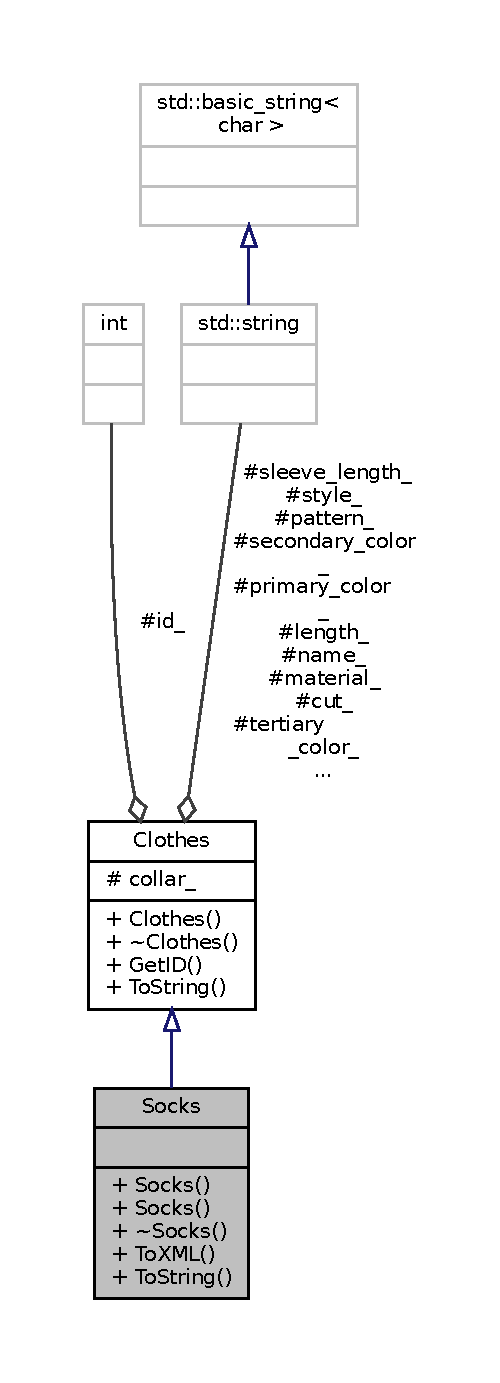
\includegraphics[height=550pt]{classSocks__coll__graph}
\end{center}
\end{figure}
\subsection*{Public Member Functions}
\begin{DoxyCompactItemize}
\item 
\mbox{\hyperlink{classSocks_a5357afba0ba13b32e1d417bdb7059c68}{Socks}} ()
\item 
\mbox{\hyperlink{classSocks_ab8f83e88b6131bbf22d75de7a41d241a}{Socks}} (int id, string name, string prim\+\_\+color, string sec\+\_\+color, string tert\+\_\+color, string pattern)
\item 
virtual \mbox{\hyperlink{classSocks_a1791f54f1b29487892245c80cbe7c50b}{$\sim$\+Socks}} ()
\item 
string \mbox{\hyperlink{classSocks_a5ecf1671277183b60f8eea7020cf32ed}{To\+X\+ML}} () const
\item 
string \mbox{\hyperlink{classSocks_aad237fbcc4ccf36a2956fcdef8760683}{To\+String}} () const
\item 
int \mbox{\hyperlink{classClothes_a3f6dac172f333126d19010f85ec44e4c}{Get\+ID}} ()
\end{DoxyCompactItemize}
\subsection*{Protected Attributes}
\begin{DoxyCompactItemize}
\item 
int \mbox{\hyperlink{classClothes_a8978d931db5ca47c3ccea30def4ae83e}{id\+\_\+}} = \mbox{\hyperlink{clothes_8h_a77186917343a417a2369cdff0bc86d31}{k\+Dummy\+ID}}
\begin{DoxyCompactList}\small\item\em Global unique identifier. \end{DoxyCompactList}\item 
string \mbox{\hyperlink{classClothes_a7f2275aaae24224d60c48af922c31b65}{name\+\_\+}} = \mbox{\hyperlink{clothes_8h_adba739b5125fd5a4066ec0ef063c0657}{k\+Dummy\+Name}}
\begin{DoxyCompactList}\small\item\em User readable name. \end{DoxyCompactList}\item 
string \mbox{\hyperlink{classClothes_a7cb005bf6cbb7f4eaa40f1b31817559c}{primary\+\_\+color\+\_\+}} = \mbox{\hyperlink{clothes_8h_a1b9c685d3bf2811d95b65e0d396c1344}{k\+Dummy\+Prim\+Color}}
\begin{DoxyCompactList}\small\item\em Primary color. \end{DoxyCompactList}\item 
string \mbox{\hyperlink{classClothes_ab8f55f67b956b25d71260cffcf273673}{secondary\+\_\+color\+\_\+}} = \mbox{\hyperlink{clothes_8h_a71c39811135425d881af7760da63a73a}{k\+Dummy\+Sec\+Color}}
\begin{DoxyCompactList}\small\item\em Secondary color. \end{DoxyCompactList}\item 
string \mbox{\hyperlink{classClothes_a3c5f1e7ab531e3ba7a38b930da8078a0}{tertiary\+\_\+color\+\_\+}} = \mbox{\hyperlink{clothes_8h_a094dde85547895fd70dafb3ab10c6783}{k\+Dummy\+Tert\+Color}}
\begin{DoxyCompactList}\small\item\em Tertiary color. \end{DoxyCompactList}\item 
string \mbox{\hyperlink{classClothes_a1d40145a4eb6d28441f112f030ab5d35}{pattern\+\_\+}} = \mbox{\hyperlink{clothes_8h_a2e72ae4d77adb7bc9cbecf4dea1e9e22}{k\+Dummy\+Pattern}}
\begin{DoxyCompactList}\small\item\em Design pattern. \end{DoxyCompactList}\item 
string \mbox{\hyperlink{classClothes_adbb9ed311f14ccbb1e4fe0e8378a95d4}{material\+\_\+}} = \mbox{\hyperlink{clothes_8h_a9df1268c6668ae4e2a728ccf032cc33d}{k\+Dummy\+Material}}
\begin{DoxyCompactList}\small\item\em Material. \end{DoxyCompactList}\item 
string \mbox{\hyperlink{classClothes_aa85ed2b95110d8c477a1aca9cb403f98}{style\+\_\+}} = \mbox{\hyperlink{clothes_8h_a9deec6ed1f40928bfa0040eeab95ed6b}{k\+Dummy\+Style}}
\begin{DoxyCompactList}\small\item\em Design style. \end{DoxyCompactList}\item 
string \mbox{\hyperlink{classClothes_ae02603eda727e33caf46ec30e761e3c3}{length\+\_\+}} = \mbox{\hyperlink{clothes_8h_a1624256dcecfb0995a74c36142593770}{k\+Dummy\+Length}}
\begin{DoxyCompactList}\small\item\em Length of the clothing. \end{DoxyCompactList}\item 
string \mbox{\hyperlink{classClothes_ac1c2286c8928a5eee91d818a098a44ac}{cut\+\_\+}} = \mbox{\hyperlink{clothes_8h_a8a6eb066049b009439505355aeaae375}{k\+Dummy\+Cut}}
\begin{DoxyCompactList}\small\item\em Cut of the clothing. \end{DoxyCompactList}\item 
string \mbox{\hyperlink{classClothes_a012aeb71e62ebaf9b5b5dd700cc8d5db}{sleeve\+\_\+length\+\_\+}} = \mbox{\hyperlink{clothes_8h_a0f53dde6a2c4c344bb7da50655497350}{k\+Dummy\+Sleeve\+Length}}
\begin{DoxyCompactList}\small\item\em Length of the sleeve. \end{DoxyCompactList}\item 
string \mbox{\hyperlink{classClothes_ae2e5026257b3a2f2ddbf61757fd3b57b}{collar\+\_\+}} = \mbox{\hyperlink{clothes_8h_ac06c9f556f68bcd2829e36c55b70a86e}{k\+Dummy\+Collar}}
\begin{DoxyCompactList}\small\item\em Type of collar. \end{DoxyCompactList}\end{DoxyCompactItemize}


\subsection{Constructor \& Destructor Documentation}
\mbox{\Hypertarget{classSocks_a5357afba0ba13b32e1d417bdb7059c68}\label{classSocks_a5357afba0ba13b32e1d417bdb7059c68}} 
\index{Socks@{Socks}!Socks@{Socks}}
\index{Socks@{Socks}!Socks@{Socks}}
\subsubsection{\texorpdfstring{Socks()}{Socks()}\hspace{0.1cm}{\footnotesize\ttfamily [1/2]}}
{\footnotesize\ttfamily Socks\+::\+Socks (\begin{DoxyParamCaption}{ }\end{DoxyParamCaption})}

\mbox{\Hypertarget{classSocks_ab8f83e88b6131bbf22d75de7a41d241a}\label{classSocks_ab8f83e88b6131bbf22d75de7a41d241a}} 
\index{Socks@{Socks}!Socks@{Socks}}
\index{Socks@{Socks}!Socks@{Socks}}
\subsubsection{\texorpdfstring{Socks()}{Socks()}\hspace{0.1cm}{\footnotesize\ttfamily [2/2]}}
{\footnotesize\ttfamily Socks\+::\+Socks (\begin{DoxyParamCaption}\item[{int}]{id,  }\item[{string}]{name,  }\item[{string}]{prim\+\_\+color,  }\item[{string}]{sec\+\_\+color,  }\item[{string}]{tert\+\_\+color,  }\item[{string}]{pattern }\end{DoxyParamCaption})}



References \mbox{\hyperlink{classClothes_a8978d931db5ca47c3ccea30def4ae83e}{Clothes\+::id\+\_\+}}, \mbox{\hyperlink{classClothes_a7f2275aaae24224d60c48af922c31b65}{Clothes\+::name\+\_\+}}, \mbox{\hyperlink{classClothes_a1d40145a4eb6d28441f112f030ab5d35}{Clothes\+::pattern\+\_\+}}, \mbox{\hyperlink{classClothes_a7cb005bf6cbb7f4eaa40f1b31817559c}{Clothes\+::primary\+\_\+color\+\_\+}}, \mbox{\hyperlink{classClothes_ab8f55f67b956b25d71260cffcf273673}{Clothes\+::secondary\+\_\+color\+\_\+}}, and \mbox{\hyperlink{classClothes_a3c5f1e7ab531e3ba7a38b930da8078a0}{Clothes\+::tertiary\+\_\+color\+\_\+}}.

\mbox{\Hypertarget{classSocks_a1791f54f1b29487892245c80cbe7c50b}\label{classSocks_a1791f54f1b29487892245c80cbe7c50b}} 
\index{Socks@{Socks}!````~Socks@{$\sim$\+Socks}}
\index{````~Socks@{$\sim$\+Socks}!Socks@{Socks}}
\subsubsection{\texorpdfstring{$\sim$\+Socks()}{~Socks()}}
{\footnotesize\ttfamily Socks\+::$\sim$\+Socks (\begin{DoxyParamCaption}{ }\end{DoxyParamCaption})\hspace{0.3cm}{\ttfamily [virtual]}}



\subsection{Member Function Documentation}
\mbox{\Hypertarget{classClothes_a3f6dac172f333126d19010f85ec44e4c}\label{classClothes_a3f6dac172f333126d19010f85ec44e4c}} 
\index{Socks@{Socks}!Get\+ID@{Get\+ID}}
\index{Get\+ID@{Get\+ID}!Socks@{Socks}}
\subsubsection{\texorpdfstring{Get\+I\+D()}{GetID()}}
{\footnotesize\ttfamily int Clothes\+::\+Get\+ID (\begin{DoxyParamCaption}{ }\end{DoxyParamCaption})\hspace{0.3cm}{\ttfamily [inline]}, {\ttfamily [inherited]}}

Here is the caller graph for this function\+:\nopagebreak
\begin{figure}[H]
\begin{center}
\leavevmode
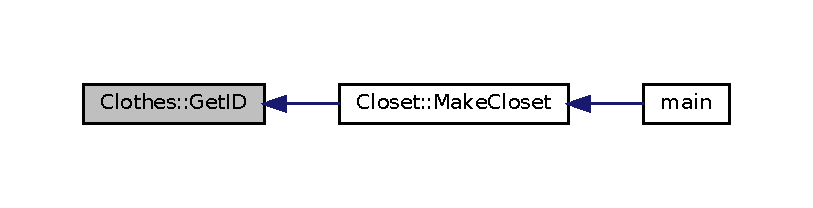
\includegraphics[width=350pt]{classClothes_a3f6dac172f333126d19010f85ec44e4c_icgraph}
\end{center}
\end{figure}
\mbox{\Hypertarget{classSocks_aad237fbcc4ccf36a2956fcdef8760683}\label{classSocks_aad237fbcc4ccf36a2956fcdef8760683}} 
\index{Socks@{Socks}!To\+String@{To\+String}}
\index{To\+String@{To\+String}!Socks@{Socks}}
\subsubsection{\texorpdfstring{To\+String()}{ToString()}}
{\footnotesize\ttfamily string Socks\+::\+To\+String (\begin{DoxyParamCaption}{ }\end{DoxyParamCaption}) const\hspace{0.3cm}{\ttfamily [virtual]}}

This is what makes this a purely abstract class. The implementation of these will be changed from one article of clothing to the next. 

Implements \mbox{\hyperlink{classClothes_a953d143394e9a2c007ab0c3a638973cf}{Clothes}}.



References \mbox{\hyperlink{classClothes_a8978d931db5ca47c3ccea30def4ae83e}{Clothes\+::id\+\_\+}}, \mbox{\hyperlink{classClothes_a7f2275aaae24224d60c48af922c31b65}{Clothes\+::name\+\_\+}}, \mbox{\hyperlink{classClothes_a1d40145a4eb6d28441f112f030ab5d35}{Clothes\+::pattern\+\_\+}}, \mbox{\hyperlink{classClothes_a7cb005bf6cbb7f4eaa40f1b31817559c}{Clothes\+::primary\+\_\+color\+\_\+}}, \mbox{\hyperlink{classClothes_ab8f55f67b956b25d71260cffcf273673}{Clothes\+::secondary\+\_\+color\+\_\+}}, and \mbox{\hyperlink{classClothes_a3c5f1e7ab531e3ba7a38b930da8078a0}{Clothes\+::tertiary\+\_\+color\+\_\+}}.

\mbox{\Hypertarget{classSocks_a5ecf1671277183b60f8eea7020cf32ed}\label{classSocks_a5ecf1671277183b60f8eea7020cf32ed}} 
\index{Socks@{Socks}!To\+X\+ML@{To\+X\+ML}}
\index{To\+X\+ML@{To\+X\+ML}!Socks@{Socks}}
\subsubsection{\texorpdfstring{To\+X\+M\+L()}{ToXML()}}
{\footnotesize\ttfamily string Socks\+::\+To\+X\+ML (\begin{DoxyParamCaption}{ }\end{DoxyParamCaption}) const}



References \mbox{\hyperlink{classClothes_a8978d931db5ca47c3ccea30def4ae83e}{Clothes\+::id\+\_\+}}, \mbox{\hyperlink{classClothes_a7f2275aaae24224d60c48af922c31b65}{Clothes\+::name\+\_\+}}, \mbox{\hyperlink{classClothes_a1d40145a4eb6d28441f112f030ab5d35}{Clothes\+::pattern\+\_\+}}, \mbox{\hyperlink{classClothes_a7cb005bf6cbb7f4eaa40f1b31817559c}{Clothes\+::primary\+\_\+color\+\_\+}}, \mbox{\hyperlink{classClothes_ab8f55f67b956b25d71260cffcf273673}{Clothes\+::secondary\+\_\+color\+\_\+}}, and \mbox{\hyperlink{classClothes_a3c5f1e7ab531e3ba7a38b930da8078a0}{Clothes\+::tertiary\+\_\+color\+\_\+}}.



\subsection{Member Data Documentation}
\mbox{\Hypertarget{classClothes_ae2e5026257b3a2f2ddbf61757fd3b57b}\label{classClothes_ae2e5026257b3a2f2ddbf61757fd3b57b}} 
\index{Socks@{Socks}!collar\+\_\+@{collar\+\_\+}}
\index{collar\+\_\+@{collar\+\_\+}!Socks@{Socks}}
\subsubsection{\texorpdfstring{collar\+\_\+}{collar\_}}
{\footnotesize\ttfamily string Clothes\+::collar\+\_\+ = \mbox{\hyperlink{clothes_8h_ac06c9f556f68bcd2829e36c55b70a86e}{k\+Dummy\+Collar}}\hspace{0.3cm}{\ttfamily [protected]}, {\ttfamily [inherited]}}



Type of collar. 

\mbox{\Hypertarget{classClothes_ac1c2286c8928a5eee91d818a098a44ac}\label{classClothes_ac1c2286c8928a5eee91d818a098a44ac}} 
\index{Socks@{Socks}!cut\+\_\+@{cut\+\_\+}}
\index{cut\+\_\+@{cut\+\_\+}!Socks@{Socks}}
\subsubsection{\texorpdfstring{cut\+\_\+}{cut\_}}
{\footnotesize\ttfamily string Clothes\+::cut\+\_\+ = \mbox{\hyperlink{clothes_8h_a8a6eb066049b009439505355aeaae375}{k\+Dummy\+Cut}}\hspace{0.3cm}{\ttfamily [protected]}, {\ttfamily [inherited]}}



Cut of the clothing. 

\mbox{\Hypertarget{classClothes_a8978d931db5ca47c3ccea30def4ae83e}\label{classClothes_a8978d931db5ca47c3ccea30def4ae83e}} 
\index{Socks@{Socks}!id\+\_\+@{id\+\_\+}}
\index{id\+\_\+@{id\+\_\+}!Socks@{Socks}}
\subsubsection{\texorpdfstring{id\+\_\+}{id\_}}
{\footnotesize\ttfamily int Clothes\+::id\+\_\+ = \mbox{\hyperlink{clothes_8h_a77186917343a417a2369cdff0bc86d31}{k\+Dummy\+ID}}\hspace{0.3cm}{\ttfamily [protected]}, {\ttfamily [inherited]}}



Global unique identifier. 

\mbox{\Hypertarget{classClothes_ae02603eda727e33caf46ec30e761e3c3}\label{classClothes_ae02603eda727e33caf46ec30e761e3c3}} 
\index{Socks@{Socks}!length\+\_\+@{length\+\_\+}}
\index{length\+\_\+@{length\+\_\+}!Socks@{Socks}}
\subsubsection{\texorpdfstring{length\+\_\+}{length\_}}
{\footnotesize\ttfamily string Clothes\+::length\+\_\+ = \mbox{\hyperlink{clothes_8h_a1624256dcecfb0995a74c36142593770}{k\+Dummy\+Length}}\hspace{0.3cm}{\ttfamily [protected]}, {\ttfamily [inherited]}}



Length of the clothing. 

\mbox{\Hypertarget{classClothes_adbb9ed311f14ccbb1e4fe0e8378a95d4}\label{classClothes_adbb9ed311f14ccbb1e4fe0e8378a95d4}} 
\index{Socks@{Socks}!material\+\_\+@{material\+\_\+}}
\index{material\+\_\+@{material\+\_\+}!Socks@{Socks}}
\subsubsection{\texorpdfstring{material\+\_\+}{material\_}}
{\footnotesize\ttfamily string Clothes\+::material\+\_\+ = \mbox{\hyperlink{clothes_8h_a9df1268c6668ae4e2a728ccf032cc33d}{k\+Dummy\+Material}}\hspace{0.3cm}{\ttfamily [protected]}, {\ttfamily [inherited]}}



Material. 

\mbox{\Hypertarget{classClothes_a7f2275aaae24224d60c48af922c31b65}\label{classClothes_a7f2275aaae24224d60c48af922c31b65}} 
\index{Socks@{Socks}!name\+\_\+@{name\+\_\+}}
\index{name\+\_\+@{name\+\_\+}!Socks@{Socks}}
\subsubsection{\texorpdfstring{name\+\_\+}{name\_}}
{\footnotesize\ttfamily string Clothes\+::name\+\_\+ = \mbox{\hyperlink{clothes_8h_adba739b5125fd5a4066ec0ef063c0657}{k\+Dummy\+Name}}\hspace{0.3cm}{\ttfamily [protected]}, {\ttfamily [inherited]}}



User readable name. 

\mbox{\Hypertarget{classClothes_a1d40145a4eb6d28441f112f030ab5d35}\label{classClothes_a1d40145a4eb6d28441f112f030ab5d35}} 
\index{Socks@{Socks}!pattern\+\_\+@{pattern\+\_\+}}
\index{pattern\+\_\+@{pattern\+\_\+}!Socks@{Socks}}
\subsubsection{\texorpdfstring{pattern\+\_\+}{pattern\_}}
{\footnotesize\ttfamily string Clothes\+::pattern\+\_\+ = \mbox{\hyperlink{clothes_8h_a2e72ae4d77adb7bc9cbecf4dea1e9e22}{k\+Dummy\+Pattern}}\hspace{0.3cm}{\ttfamily [protected]}, {\ttfamily [inherited]}}



Design pattern. 

\mbox{\Hypertarget{classClothes_a7cb005bf6cbb7f4eaa40f1b31817559c}\label{classClothes_a7cb005bf6cbb7f4eaa40f1b31817559c}} 
\index{Socks@{Socks}!primary\+\_\+color\+\_\+@{primary\+\_\+color\+\_\+}}
\index{primary\+\_\+color\+\_\+@{primary\+\_\+color\+\_\+}!Socks@{Socks}}
\subsubsection{\texorpdfstring{primary\+\_\+color\+\_\+}{primary\_color\_}}
{\footnotesize\ttfamily string Clothes\+::primary\+\_\+color\+\_\+ = \mbox{\hyperlink{clothes_8h_a1b9c685d3bf2811d95b65e0d396c1344}{k\+Dummy\+Prim\+Color}}\hspace{0.3cm}{\ttfamily [protected]}, {\ttfamily [inherited]}}



Primary color. 

\mbox{\Hypertarget{classClothes_ab8f55f67b956b25d71260cffcf273673}\label{classClothes_ab8f55f67b956b25d71260cffcf273673}} 
\index{Socks@{Socks}!secondary\+\_\+color\+\_\+@{secondary\+\_\+color\+\_\+}}
\index{secondary\+\_\+color\+\_\+@{secondary\+\_\+color\+\_\+}!Socks@{Socks}}
\subsubsection{\texorpdfstring{secondary\+\_\+color\+\_\+}{secondary\_color\_}}
{\footnotesize\ttfamily string Clothes\+::secondary\+\_\+color\+\_\+ = \mbox{\hyperlink{clothes_8h_a71c39811135425d881af7760da63a73a}{k\+Dummy\+Sec\+Color}}\hspace{0.3cm}{\ttfamily [protected]}, {\ttfamily [inherited]}}



Secondary color. 

\mbox{\Hypertarget{classClothes_a012aeb71e62ebaf9b5b5dd700cc8d5db}\label{classClothes_a012aeb71e62ebaf9b5b5dd700cc8d5db}} 
\index{Socks@{Socks}!sleeve\+\_\+length\+\_\+@{sleeve\+\_\+length\+\_\+}}
\index{sleeve\+\_\+length\+\_\+@{sleeve\+\_\+length\+\_\+}!Socks@{Socks}}
\subsubsection{\texorpdfstring{sleeve\+\_\+length\+\_\+}{sleeve\_length\_}}
{\footnotesize\ttfamily string Clothes\+::sleeve\+\_\+length\+\_\+ = \mbox{\hyperlink{clothes_8h_a0f53dde6a2c4c344bb7da50655497350}{k\+Dummy\+Sleeve\+Length}}\hspace{0.3cm}{\ttfamily [protected]}, {\ttfamily [inherited]}}



Length of the sleeve. 

\mbox{\Hypertarget{classClothes_aa85ed2b95110d8c477a1aca9cb403f98}\label{classClothes_aa85ed2b95110d8c477a1aca9cb403f98}} 
\index{Socks@{Socks}!style\+\_\+@{style\+\_\+}}
\index{style\+\_\+@{style\+\_\+}!Socks@{Socks}}
\subsubsection{\texorpdfstring{style\+\_\+}{style\_}}
{\footnotesize\ttfamily string Clothes\+::style\+\_\+ = \mbox{\hyperlink{clothes_8h_a9deec6ed1f40928bfa0040eeab95ed6b}{k\+Dummy\+Style}}\hspace{0.3cm}{\ttfamily [protected]}, {\ttfamily [inherited]}}



Design style. 

\mbox{\Hypertarget{classClothes_a3c5f1e7ab531e3ba7a38b930da8078a0}\label{classClothes_a3c5f1e7ab531e3ba7a38b930da8078a0}} 
\index{Socks@{Socks}!tertiary\+\_\+color\+\_\+@{tertiary\+\_\+color\+\_\+}}
\index{tertiary\+\_\+color\+\_\+@{tertiary\+\_\+color\+\_\+}!Socks@{Socks}}
\subsubsection{\texorpdfstring{tertiary\+\_\+color\+\_\+}{tertiary\_color\_}}
{\footnotesize\ttfamily string Clothes\+::tertiary\+\_\+color\+\_\+ = \mbox{\hyperlink{clothes_8h_a094dde85547895fd70dafb3ab10c6783}{k\+Dummy\+Tert\+Color}}\hspace{0.3cm}{\ttfamily [protected]}, {\ttfamily [inherited]}}



Tertiary color. 



The documentation for this class was generated from the following files\+:\begin{DoxyCompactItemize}
\item 
\mbox{\hyperlink{socks_8h}{socks.\+h}}\item 
\mbox{\hyperlink{socks_8cc}{socks.\+cc}}\end{DoxyCompactItemize}

\hypertarget{classVulkan}{}\section{Vulkan Class Reference}
\label{classVulkan}\index{Vulkan@{Vulkan}}


{\ttfamily \#include $<$vulkan.\+h$>$}



Collaboration diagram for Vulkan\+:\nopagebreak
\begin{figure}[H]
\begin{center}
\leavevmode
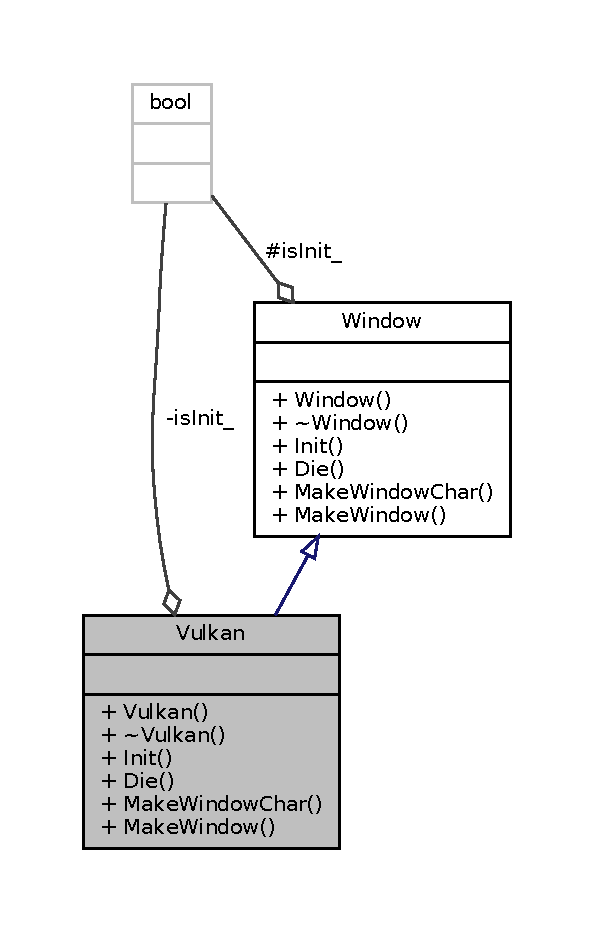
\includegraphics[width=203pt]{classVulkan__coll__graph}
\end{center}
\end{figure}
\subsection*{Public Member Functions}
\begin{DoxyCompactItemize}
\item 
\mbox{\hyperlink{classVulkan_a69c8a0222ecd2f24887acc75a7ffd922}{Vulkan}} ()
\item 
virtual \mbox{\hyperlink{classVulkan_a85f20d6cd141ec9568d812cfdf81971f}{$\sim$\+Vulkan}} ()
\item 
bool \mbox{\hyperlink{classVulkan_a308c68e03405bc740435a2af62cc7434}{Init}} ()
\item 
void \mbox{\hyperlink{classVulkan_a728e47da1e42d65c6d9efa5106f6d13b}{Die}} ()
\item 
char \mbox{\hyperlink{classVulkan_a70565678cd6771ac57706ff8586e256f}{Make\+Window\+Char}} (string message)
\item 
string \mbox{\hyperlink{classVulkan_a46c4ec53f8960a1fa3f3eb63d7755654}{Make\+Window}} (string message)
\end{DoxyCompactItemize}
\subsection*{Private Attributes}
\begin{DoxyCompactItemize}
\item 
bool \mbox{\hyperlink{classVulkan_aa19833e837744cc2f6b1f93c1d66a693}{is\+Init\+\_\+}} = false
\end{DoxyCompactItemize}


\subsection{Constructor \& Destructor Documentation}
\mbox{\Hypertarget{classVulkan_a69c8a0222ecd2f24887acc75a7ffd922}\label{classVulkan_a69c8a0222ecd2f24887acc75a7ffd922}} 
\index{Vulkan@{Vulkan}!Vulkan@{Vulkan}}
\index{Vulkan@{Vulkan}!Vulkan@{Vulkan}}
\subsubsection{\texorpdfstring{Vulkan()}{Vulkan()}}
{\footnotesize\ttfamily Vulkan\+::\+Vulkan (\begin{DoxyParamCaption}{ }\end{DoxyParamCaption})}

\mbox{\Hypertarget{classVulkan_a85f20d6cd141ec9568d812cfdf81971f}\label{classVulkan_a85f20d6cd141ec9568d812cfdf81971f}} 
\index{Vulkan@{Vulkan}!````~Vulkan@{$\sim$\+Vulkan}}
\index{````~Vulkan@{$\sim$\+Vulkan}!Vulkan@{Vulkan}}
\subsubsection{\texorpdfstring{$\sim$\+Vulkan()}{~Vulkan()}}
{\footnotesize\ttfamily Vulkan\+::$\sim$\+Vulkan (\begin{DoxyParamCaption}{ }\end{DoxyParamCaption})\hspace{0.3cm}{\ttfamily [virtual]}}



\subsection{Member Function Documentation}
\mbox{\Hypertarget{classVulkan_a728e47da1e42d65c6d9efa5106f6d13b}\label{classVulkan_a728e47da1e42d65c6d9efa5106f6d13b}} 
\index{Vulkan@{Vulkan}!Die@{Die}}
\index{Die@{Die}!Vulkan@{Vulkan}}
\subsubsection{\texorpdfstring{Die()}{Die()}}
{\footnotesize\ttfamily void Vulkan\+::\+Die (\begin{DoxyParamCaption}{ }\end{DoxyParamCaption})}

\mbox{\Hypertarget{classVulkan_a308c68e03405bc740435a2af62cc7434}\label{classVulkan_a308c68e03405bc740435a2af62cc7434}} 
\index{Vulkan@{Vulkan}!Init@{Init}}
\index{Init@{Init}!Vulkan@{Vulkan}}
\subsubsection{\texorpdfstring{Init()}{Init()}}
{\footnotesize\ttfamily bool Vulkan\+::\+Init (\begin{DoxyParamCaption}{ }\end{DoxyParamCaption})}

\mbox{\Hypertarget{classVulkan_a46c4ec53f8960a1fa3f3eb63d7755654}\label{classVulkan_a46c4ec53f8960a1fa3f3eb63d7755654}} 
\index{Vulkan@{Vulkan}!Make\+Window@{Make\+Window}}
\index{Make\+Window@{Make\+Window}!Vulkan@{Vulkan}}
\subsubsection{\texorpdfstring{Make\+Window()}{MakeWindow()}}
{\footnotesize\ttfamily string Vulkan\+::\+Make\+Window (\begin{DoxyParamCaption}\item[{string}]{message }\end{DoxyParamCaption})}

\mbox{\Hypertarget{classVulkan_a70565678cd6771ac57706ff8586e256f}\label{classVulkan_a70565678cd6771ac57706ff8586e256f}} 
\index{Vulkan@{Vulkan}!Make\+Window\+Char@{Make\+Window\+Char}}
\index{Make\+Window\+Char@{Make\+Window\+Char}!Vulkan@{Vulkan}}
\subsubsection{\texorpdfstring{Make\+Window\+Char()}{MakeWindowChar()}}
{\footnotesize\ttfamily char Vulkan\+::\+Make\+Window\+Char (\begin{DoxyParamCaption}\item[{string}]{message }\end{DoxyParamCaption})}



\subsection{Member Data Documentation}
\mbox{\Hypertarget{classVulkan_aa19833e837744cc2f6b1f93c1d66a693}\label{classVulkan_aa19833e837744cc2f6b1f93c1d66a693}} 
\index{Vulkan@{Vulkan}!is\+Init\+\_\+@{is\+Init\+\_\+}}
\index{is\+Init\+\_\+@{is\+Init\+\_\+}!Vulkan@{Vulkan}}
\subsubsection{\texorpdfstring{is\+Init\+\_\+}{isInit\_}}
{\footnotesize\ttfamily bool Vulkan\+::is\+Init\+\_\+ = false\hspace{0.3cm}{\ttfamily [private]}}



The documentation for this class was generated from the following files\+:\begin{DoxyCompactItemize}
\item 
\mbox{\hyperlink{vulkan_8h}{vulkan.\+h}}\item 
\mbox{\hyperlink{vulkan_8cc}{vulkan.\+cc}}\end{DoxyCompactItemize}

\hypertarget{classWindow}{}\section{Window Class Reference}
\label{classWindow}\index{Window@{Window}}
\subsection*{Public Member Functions}
\begin{DoxyCompactItemize}
\item 
\mbox{\Hypertarget{classWindow_a91ad1340d4f60465f0e6eef38f0e5fb1}\label{classWindow_a91ad1340d4f60465f0e6eef38f0e5fb1}} 
virtual bool {\bfseries Init} ()=0
\item 
\mbox{\Hypertarget{classWindow_a5332552d06a88b58486c0ab803356d01}\label{classWindow_a5332552d06a88b58486c0ab803356d01}} 
virtual void {\bfseries Die} ()=0
\item 
\mbox{\Hypertarget{classWindow_ae770439748fb6b7dcdb3071860e687b3}\label{classWindow_ae770439748fb6b7dcdb3071860e687b3}} 
virtual char {\bfseries Make\+Window\+Char} (string message)=0
\item 
\mbox{\Hypertarget{classWindow_a3a24c6368cb054a5ca3b32db2558319f}\label{classWindow_a3a24c6368cb054a5ca3b32db2558319f}} 
virtual string {\bfseries Make\+Window} (string message)=0
\end{DoxyCompactItemize}
\subsection*{Protected Attributes}
\begin{DoxyCompactItemize}
\item 
\mbox{\Hypertarget{classWindow_a06739ea2d178febdb7f0da5f775e5ba8}\label{classWindow_a06739ea2d178febdb7f0da5f775e5ba8}} 
bool {\bfseries is\+Init\+\_\+} = false
\end{DoxyCompactItemize}


The documentation for this class was generated from the following file\+:\begin{DoxyCompactItemize}
\item 
window.\+h\end{DoxyCompactItemize}

%--- End generated contents ---

% Index
\backmatter
\newpage
\phantomsection
\clearemptydoublepage
\addcontentsline{toc}{chapter}{Index}
\printindex

\end{document}
